\documentclass[oneside,12pt,numbers,spanish]{ezthesis}
%% # Opciones disponibles para el documento #
%%
%% Las opciones con un (*) son las opciones predeterminadas.
%%
%% Modo de compilar:
%%   draft            - borrador con marcas de fecha y sin im'agenes
%%   draftmarks       - borrador con marcas de fecha y con im'agenes
%%   final (*)        - version final de la tesis
%%
%% Tama'no de papel:
%%   letterpaper (*)  - tama'no carta (Am'erica)
 %%   a4paper          - tama'no A4    (Europa)
%%
%% Formato de impresi'on:
%%   oneside          - hojas impresas por un solo lado
%%   twoside (*)      - hijas impresas por ambos lados
%%
%% Tama'no de letra:
%%   10pt, 11pt, o 12pt (*)
%%
%% Espaciado entre renglones:
%%   singlespace      - espacio sencillo
%%   onehalfspace (*) - espacio de 1.5
%%   doublespace      - a doble espacio
%%
%% Formato de las referencias bibliogr'aficas:
%%   numbers          - numeradas, p.e. [1]
%%   authoryear (*)   - por autor y a'no, p.e. (Newton, 1997)
%%
%% Opciones adicionales:
%%   spanish         - tesis escrita en espa'nol
%%
%% Desactivar opciones especiales:
%%   nobibtoc   - no incluir la bibiolgraf'ia en el 'Indice general
%%   nofancyhdr - no incluir "fancyhdr" para producir los encabezados
%%   nocolors   - no incluir "xcolor" para producir ligas con colores
%%   nographicx - no incluir "graphicx" para insertar gr'aficos
%%   nonatbib   - no incluir "natbib" para administrar la bibliograf'ia

%% Paquetes adicionales requeridos se pueden agregar tambi'en aqu'i.
%% Por ejemplo:
\usepackage[spanish]{babel}
\usepackage{cite}
\usepackage{natbib} 
\usepackage{subfig}
\usepackage[utf8x]{inputenc}
\usepackage{multicol}
\usepackage{multirow, array}
\usepackage{graphicx} 
\usepackage{float}  
\usepackage{amsmath}
\usepackage{amssymb}
\usepackage{pgfgantt}


%% # Datos del documento #
%%\documentclass[12pt]{•}%% Nota que los acentos se deben escribir: \'a, \'e, \'i, etc.
%% La letra n con tilde es: \~n.

\author{Jesús David Escalante Rodr\'iguez}
\title{Paquete en lenguaje R para la clasificaci\'on de tub\'erculos de papa criolla(\textit{Solanum phureja}) para diferentes densidades de siembra empleando redes neuronales probabil\'isticas.}
\supervisor{ Rossana Timaure}
\institution{Universidad Nacional Experimental del T\'achira}
\faculty{Vicerectorado Acad\'emico}
\department{Departamento de Ingeniería en Informática}

\pretolerance = 2000
\tolerance = 3000
\righthyphenmin = 2000
\lefthyphenmin = 2000
%% # M'argenes del documento #
%% 
%% Quitar el comentario en la siguiente linea para austar los m'argenes del
%% documento. Leer la documentaci'on de "geometry" para m'as informaci'on.

\geometry{left=2cm,right=2cm,top=3cm,bottom=3cm}

%% El siguiente comando agrega ligas activas en el documento para las
%% referencias cruzadas y citas bibliogr'aficas. Tiene que ser *la 'ultima*
%% instrucci'on antes de \begin{document}.
\hyperlinking
\begin{document}

%% En esta secci'on se describe la estructura del documento de la tesis.
%% Consulta los reglamentos de tu universidad para determinar el orden
%% y la cantidad de secciones que debes de incluir.

%% # Portada de la tesis #
%% Mirar el archivo "titlepage.tex" para los detalles.
%% ## Construye tu propia portada ##
%% 
%% Una portada se conforma por una secuencia de "Blocks" que incluyen
%% piezas individuales de informaci'on. Un "Block" puede incluir, por
%% ejemplo, el t'itulo del documento, una im'agen (logotipo de la universidad),
%% el nombre del autor, nombre del supervisor, u cualquier otra pieza de
%% informaci'on.
%%
%% Cada "Block" aparece centrado horizontalmente en la p'agina y,
%% verticalmente, todos los "Blocks" se distruyen de manera uniforme 
%% a lo largo de p'agina.
%%
%% Nota tambi'en que, dentro de un mismo "Block" se pueden cortar
%% lineas usando el comando \\
%%
%% El tama'no del texto dentro de un "Block" se puede modificar usando uno de
%% los comandos:
%%   \small      \LARGE
%%   \large      \huge
%%   \Large      \Huge
%%
%% Y el tipo de letra se puede modificar usando:
%%   \bfseries - negritas
%%   \itshape  - it'alicas
%%   \scshape  - small caps
%%   \slshape  - slanted
%%   \sffamily - sans serif
%%
%% Para producir plantillas generales, la informaci'on que ha sido inclu'ida
%% en el archivo principal "tesis.tex" se puede accesar aqu'i usando:
%%   \insertauthor
%%   \inserttitle
%%   \insertsupervisor
%%   \insertinstitution
%%   \insertdegree
%%   \insertfaculty
%%   \insertdepartment
%%   \insertsubmitdate

\begin{titlepage}
  \TitleBlock{
\includegraphics[scale=0.2]{unet.jpg} }  
  \TitleBlock{\small\insertinstitution}
  \TitleBlock[\small\bigskip]{\insertfaculty}
  \TitleBlock[\small\bigskip]{Decanato de Docencia}
  \TitleBlock[\small\bigskip]{\insertdepartment}
  \TitleBlock[\small\bigskip]{Trabajo de aplicaci\'on profesional}
  \TitleBlock[\small\bigskip]{Proyecto especial de grado}
    
 \TitleBlock{\scshape\inserttitle}
 
 \begin{flushright}
  \TitleBlock{ \small Autor(es):  \insertauthor} 
  \TitleBlock{ \small C.I.: 21.220.841}
  \TitleBlock{ \small jesusd.escalante@unet.edu.ve}
  \TitleBlock{\small Tutor(es):  \insertsupervisor}
  \TitleBlock{ \small rttg@unet.edu.ve}
 \end{flushright}
  \TitleBlock{\small San Crist\'obal, Julio de 2018.\insertsubmitdate}
  
\end{titlepage}

%% Nota 1:
%% Se puede agregar un escudo o logotipo en un "Block" como:
%%   \TitleBlock{\includegraphics[height=4cm]{escudo_uni}}
%% y teniendo un archivo "escudo_uni.pdf", "escudo_uni.png" o "escudo_uni.jpg"
%% en alg'un lugar donde LaTeX lo pueda encontrar.

%% Nota 2:
%% Normalmente, el espacio entre "Blocks" se extiende de modo que el
%% contenido se reparte uniformemente sobre toda la p'agina. Este
%% comportamiento se puede modificar para mantener fijo, por ejemplo, el
%% espacio entre un par de "Blocks". Escribiendo:
%%   \TitleBlock{Bloque 1}
%%   \TitleBlock[\bigskip]{Bloque2}
%% se deja un espacio "grande" y de tama~no fijo entre el bloque 1 y 2.
%% Adem'as de \bigskip est'an tambi'en \smallskip y \medskip. Si necesitas
%% aun m'as control puedes usar tambi'en, por ejemplo, \vspace*{2cm}.



\tableofcontents
% \listoffigures


\chapter*{Introducci\'on}
\pagenumbering{arabic} % para empezar la numeración con números

En los cultivos de papa criolla son muchas las variables que influyen en la cosecha de tub\'erculos, tales como la temperatura, altura del terreno, clima, tipo y composici\'on del suelo, densidad de siembra, entre otros y las personas interesadas en este proceso siempre han buscado manipularlas para no solo mejorar la calidad del producto, si no para obtenerlo con ciertas caracter\'isticas que sean convenientes para su fin, como por ejemplo la piel, contextura, pero muy sobre todo el tama\~no de los tub\'erculos ya que existen diferentes intereses industriales en esta \'ultima caracter\'istica.\\

Investigaciones anteriores concluyeron que la densidad de siembra es una variable con una afectaci\'on considerable en el tama\~no de los tub\'erculos producidos por las plantas en su ciclo de cosecha, sin embargo la manipulaci\'on de esta variable en dichas investigaci\'ones fue de tipo lineal, sin tener en cuenta ciertas condiciones espaciales que posee como propiedades esta variable, por la misma representar la distancia entre calles y surcos, y distancia entre plantas a la que se siembra, o expresado de otra manera cuantas plantas son sembradas por metro cuadrado en un terreno. La densidad de siembra es una variable cualitativa que aunque se trata de distancias se define en densidades predeterminadas como d1 = 50x30cm, donde d1 es una densidad definida igual a un espacio entre surcos de 50cm y distancia entre plantas de 30cm.\\

El objetivo de esta investigaci\'on es construir un paquete en Lenguaje R que permita a trav\'es de una entrada, propuesta como una matriz cargada con los datos observados de cultivo, clasificar los tub\'erculos de papa criolla cosechados en densidades de siembra seg\'un el peso total del cultivo, peso total de tub\'erculos y diam\'etro de cada tub\'erculo a trav\'es de una red neuronal probabil\'istica entrenada con datos del cultivo anteriormente recogidos. La red neuronal se encargar\'a de clasificar basado en sus neuronas entrenadas a trav\'es de datos conocidos con anterioridad por lo que no es de importancia el hecho de que no exista una relacion entre estas variables ya que no requiere de supuestos estad\'isticos para realizar el proceso de clasificaci\'on. Los datos que ser\'an usados en la presente investigaci\'on fueron recogidos y observados de la cosecha de un cultivo de tub\'erculos de papa criolla realizado en el Centro Agropecuario Marengo de la Universidad Nacional de Colombia, en el departamento de Cundinamarca en Colombia (74°12'58.51''W;4°40'52.92''N), el cual tiene una altitud de 2516 msnm y una temperatura media de 14 °C.\\
 


\chapter{Preliminares}

\section{Planteamiento y formulación del problema}

La producción de papa criolla (\textit{S. phureja}), siempre ha tenido muchos desafíos por parte de la industria, debido a los grandes intereses provenientes de los diferentes consumidores que la misma posee, siendo así que es uno de los productos agr\'icolas mas consumidos y con mayor importancia en el mundo, después del arroz, el ma\'iz y el trigo. Colombia es el mayor productor de papa criolla en Latinoamerica y por lo cual es un pa\'is que posee grandes exigencias industriales para su producción (Ligarreto \textit{et al.}, 2003).\\

Los tubérculos de papa criolla tienen un tamaño aproximado entre dos y ocho centímetros (2-8 cm), y se pueden clasificar en tres calibres según su diámetro transversal promedio,  de donde radican los intereses comerciales de la misma. Los tubérculos de entre dos y medio y cuatro centímetros son preferidos para encurtidos y pre-cocidos mientras los tubérculos promedio entre cuatro y seis y medio centímetros son preferidos para frituras en hojuelas o con mas de cinco centímetros para frituras en tiras (CORPOICA, 2009).\\

El crecimiento vegetal es definido  como el aumento irreversible del tamaño y peso seco de las plantas (altura, área foliar, diámetro, número de células y cantidad de protoplasma) o los cambios que ocurren en una planta o población de plantas a través del tiempo, fenómeno acompañado del aumento en la complejidad estructural metabólica del organismo (diferenciación celular, número de hojas), por procesos de división y alargamiento celular, incorporación de materia y energía del ambiente (fotosíntesis, absorción de agua y de iones) y metabolización subsiguiente (Cabezas 2005), la cual se traduce en multiplicación y diferenciación celular. Este proceso está íntimamente relacionado con algunos factores internos como fotosíntesis, respiración, transpiración, condiciones de estrés, concentración enzimática, balance hormonal y expresión genética(Piñeros, 2009).\\

En la papa son dos los procesos fisiológicos asociados directamente al rendimiento de la misma, la fotosíntesis y la respiración. Y estos dos son procesos íntimamente asociados, ya que durante la fotosíntesis se producen carbohidratos que son consumidos durante la respiración, pero una gran cantidad de estos carbohidratos contribuyen al proceso de producción incrementando el tamaño de los tubérculos, el nivel y periodo de crecimiento de los tubérculos es una variable que responde directamente a la expresión de rendimiento expresada como producción por día, siendo así que cerca de un noventa por ciento (90\%) del peso acumulado de los tubérculos producidos por una planta es producto de la asimilación de dióxido de carbono, así como otros procesos similares (Beukema, 1979). Sin embargo, estos procesos se ven afectados por condiciones externas tales como la intensidad de luz, temperatura, longitud de los días, condiciones del suelo que son variables no controladas, o por condiciones como la cantidad de riego, fertilizantes aplicados para la mejora de los suelos que son variables controlables pero que requieren de costos adicionales de producción (Pineros, 2009). Es por ello que se sigue buscando, con el manejo de variables controladas,  el control sobre la cantidad total producida y el tamaño de los tubérculos,  sin producir costos adicionales, siendo la densidad de siembra una de estas variables, en la cual nos enfocaremos en esta investigación (Bernal, 2017).\\

Sin embargo,  la densidad de siembra es una variable de tipo espacial, ya que se define como la distancia entre plantas y entre linderas, siendo así una coordenada en X - Y en un plano cartesiano, por lo cual un estudio estadístico de la misma para clasificar o predecir un modelo no puede ser del tipo de regresión lineal o de un análisis de varianza,  debido a que los supuestos de estos modelos establecen que los residuales deben ser independientes en cada punto, no tomando en cuenta una relación entre vecinos, como si ocurre en los cultivos de papa, las plantas compiten por los recursos y por consiguiente por producir más, haciendo así los residuales dependientes  (Pi\~neros, 2009). \\

La identificación siempre ha sido un problema de interés en el área agrícola, existen trabajos sobre la identificación de variedades de papas, sobre la capacidad de las plantas de papas para cobertura del suelo entre otras variables de estudio sometidas a clasificación, esto debido al impacto que tiene la comercialización y manejo agrícola del producto, entre las técnicas empleadas se encuentran modelos estadísticos basados en probabilidad, las máquinas de soporte vectorial y las redes neuronales, estas últimas técnicas presentan la ventaja de que bajo el proceso de aprendizaje supervisado no presentan supuestos rígidos en cuanto al comportamiento y relación de los datos de entrada (Pal, 2003; Aziz 2016).\\

Una red neuronal artificial (\textit{artificial neural network}, ANN) es un modelo que crea una relación entre una configuración de señales de entrada y una señal de salida usando un modelo derivado de nuestro entendimiento de como el cerebro responde a determinados estímulos de entradas sensoriales. Así como un cerebro usa ese conjunto de células interconectadas llamadas neuronas, así las ANN usan una red de neuronal artificiales o nodos para solucionar problemas aprendidos (Lantz, 2015).\\

En general, las ANN son aprendices versátiles que pueden ser aplicadas a casi cualquier tarea de aprendizaje en cualquier contexto, clasificación, predicción, reconocimiento de patrones e incluso  de tareas de supervisión de procesos. Las ANN, se aplican mejor a los problemas cuyos datos de entrada y salida son bien definidos o bastante simples, sin embargo el proceso que relaciona la entrada con una determinada salida es en extremo complejo, por eso se conocen como un método de caja negra (Lantz, 2015).\\

Las ANN han sido usadas desde hace cincuenta años para simular como el cerebro humano es capaz de resolver problemas. Primero surgieron las simples funciones lógicas AND y OR, que ayudaron a los científicos a entender como biológicamente el cerebro opera. Sin embargo, como el avance tecnológico y computacional ha sido incrementado y continua creciendo potencialmente durante los últimos años, las ANN ha incrementado su complejidad siendo usadas frecuentemente en múltiples problemas como:

\begin{enumerate}
    \item{Programas de reconocimiento de voz y escritura, como los que usan los correo de voz
de los servicios de transcripción y máquinas clasificadoras de correo postal.}
	\item{La automatización de dispositivos inteligentes como los controles ambientales de un edificio de oficinas o automóviles autodirigidos y drones autoguiados.}
	\item{Modelos sofisticados de patrones climáticos y otros fenómenos científicos, sociales o económicos.}
	\item{La clasificaci\'on y reconocimiento de cualquier tipo de frutos y hojas de plantas, basado en sus atributos y características.}
\end{enumerate} 

Las redes neuronales probabilísticas  (\textit{Probabilistic neural network}, PNN) se derivan de las ANN y se diferencian en que estas hacen uso de redes de funciones de base radial. Son adoptadas en muchos casos por su fácil entrenamiento y velocidad de análisis. Las PNN tienen tres capas, una primera de entrada, una de base radial y otra de competición. Básicamente la capa de base radial evalúa las distancias entre los valores de un vector de entrada y estas distancias son escaladas no linealmente, para que la capa de competitividad encuentre las distancia mas corta , a través de la cual realiza la clasificación.\\

R es un lenguaje de programación y entornos para gráficos y c\'alculos estad\'isticos, es una implementación diferente al lenguaje S (Chambers, 1998), y se desarrolla bajo un proyecto de \textit{software} bajo Licencia Pública General (\textit{General Public License}, GNU) de la \textit{Free Software Foundation} (\url{https://www.fsf.org/}) en forma de codigo fuente. Se compila y se ejecuta en una amplia variedad de plataformas entre ellas \textit{FreeBSD},\textit{Linux}, \textit{Windows} y\textit{MacOS}. (The R Project for Statistical Computing, 2018).\\


Esta propuesta tiene como objetivo desarrollar un paquete en lenguaje R que permita ajustar y entrenar una red neuronal artificial probabil\'istica para la clasificación de densidades de siembra de papa criolla (\textit{Solanum Phureja}) teniendo como entrada las siguientes variables: 

\begin{enumerate}
    \item{\textbf{Peso total del cultivo.} Variable cuantitativa expresada en gramos (g/cosecha), que indica el peso de todos los tubérculos recogidos en la siembra.}
	\item{\textbf{Total de tubérculos recogidos.} Variable cuantitativa que indica el número/cosecha de tubérculos recogidos en la siembra.}
	\item{\textbf{Diámetro ponderado de todos los tubérculos.} Variable cuantitativa expresada en centímetros (cm.), que indica el calculo del diámetro ponderado (por los tubérculos ser ovoides) de cada tubérculo recogido en la siembra.}
\end{enumerate}


Esta herramienta permitirá entre otras cosas a investigadores del área agrícola y a bioestadísticos comparar los resultados de clasificación alimentando la red con datos observados y con los mismos datos normalizados especialmente a través de regresión espacial, para observar si es necesario el análisis de los datos recogidos antes de la clasificación y a su vez concluir hasta que punto la densidad de siembra afecta las variables antes mencionadas. Otra de las pruebas que se plantea usar en esta investigación es realizar los análisis eliminando variables de entrada atisbando cuales variables permiten y generan una mejor clasificación.\\

\section{Objetivos}

\subsection{Objetivo General}

Desarrollar un paquete en lenguaje R que permita la clasificación de tubérculos de papa criolla (\textit{S. phureja}) para diferentes densidades de siembra empleando redes neuronales probabilísticas.

\subsection{Objetivos Espec\'ificos}
 
\begin{itemize}
\item{Estudiar la parametrizaci\'on de la densidad de siembra como par\'ametro de entrada al clasificador}
\item{Diseñar los algoritmos para las funciones principales que permitan el entrenamiento de una red neuronal probabilística para la clasificación de tubérculos de papa criolla (\textit{S. phureja}) para diferentes densidades de siembra.}
\item{Implementar las funciones  para la clasificación de tubérculos de papa criolla para diferentes densidades de siembra, basadas en los algorítmos desarrollados.}
\item{Realizar la pruebas del paquete desarrollado bajo diferente escenarios.}
\end{itemize}

\section{Justificación e Importancia}

Colombia es el mayor productor, consumidor y exportador de papas diploides en el mundo; tiene una ventaja competitiva notable debido a ser centro de diversidad y poseer gran aceptación por los consumidores debido a las características del tubérculo. Adicionalmente, en este país se ha desarrollado una amplia tradición como cultivo tecnificado, con potencial de industrialización y exportación (Rodríguez \textit{et al}, 2009). Ademas de contar con uno de los recursos genéticos que ofrece las mayores oportunidades de exportación como alimento procesado exclusivo y sin competencia. Desafortunadamente, muchas de las estrategias de manejo del cultivo de la papa, han sido adaptadas a papa criolla (\textit{S. phureja}), creando un sistema productivo poco eficiente (Piñeros, 2009). Los altos precios de los insumos agrícolas y el mal manejo de los cultivos agronómicamente provoca  baja productividad y amenaza la competitividad del sistema de producción, por lo que es importante identificar factores limitantes del rendimiento y desarrollar practicas innovadoras para el cultivo, tales como una gestión nutricional integrada y equilibrada, que es una de las practicas mas eficientes para garantizar a la planta la oportunidad de expresar su potencial genético que eventualmente se reflejara en una mejor calidad y rendimiento (López \textit{et al}, 2014).\\
 
Varias investigaciones revelan que el tamaño promedio de los tubérculos, su variabilidad y su conteo, definen una única distribución, presentando mayor variabilidad de rangos de tamaño en la etapa final de llenado, con aumento del rendimiento de los mayores tamaños por cuenta de los tamaños inferiores, lo que sugiere que un tubérculo que pasa de un calibre inferior al siguiente, no es sustituido por otro de calibre anterior, además, parece existir una correlación negativa entre la variabilidad relativa del tamaño del tubérculo y el número de tubérculos por unidad de área (Struik, 1991).\\

Es importante reconocer, que debe tenerse cuidado con la interpretación de esta correlación, pues hasta cierto punto, la naturaleza de los datos asociados al número de tubérculos por planta pudiera ser similar a la de los datos composicionales, es decir, si un componente aumenta, el otro esta forzado a disminuir, lo que genera correlaciones sin conexión lógica en datos verdaderamente composicionales, sin embargo, el número de tubérculos por calibre no suma una constante, pudiera ocurrir que su máximo posea una distribución específica, entonces una mayor cantidad de tubérculos de un calibre podría provocar un número menor de tubérculos en otro calibre especifico, lo que en esencia puede generar correlaciones en las que debe tenerse mucho cuidado al momento de su interpretación.\\

 La importancia del cultivo obliga a muchos investigadores a realizar diferentes estudios para mejorar la práctica agrícola, la descripción y clasificación de las variables que impacten en el estudio del crecimiento de los tubérculos, ya que de eso depende el uso a darles;   procurando siempre hacer uso del espacio de siembra de forma óptima, por lo que varios estudios evidencian el estudio de la densidad de siembra para evaluar sobre todo el rendimiento. En  Bernal(2017) evaluó en lugar del rendimiento, un indicador que se asocia directamente como lo es el calibre de los tubérculos, los cuales en la práctica se manipulan en cuatro categorías de diámetro promedio (hasta 2 cm, de 2 a 4 cm, de 4 a 6 cm y más de 6 cm). La naturaleza de esta variable imposibilita usualmente la comparación de la respuesta (conteos de tubérculos) para cada densidad de siembra (definidas como 30cm*100cm, 40cm*100cm y 50cm*100cm) mediante análisis de varianza, pues en el caso de conteos, otras distribuciones como la Poisson y la Binomial negativa se adaptan mucho mejor al tipo de dato generado. Los modelos clásicos de regresión Poisson y binomial y negativa, en sus modalidades usuales o en la opción inflada por ceros (Cameron, 1998) en datos de conteo pertenecen a la familia de modelos lineales generalizados (Zeileis, 2008) y los desarrollos recientes permiten generar varias estadísticas que permiten su comparación con sus contrapartes sin ceros en exceso, lo que resulta útil en la elección del mejor modelo para relacionar predictores y respuesta en conteos.\\

Sin embargo, los estudios realizados hasta ahora son todos haciendo suposiciones del tipo lineal y haciendo modificaciones que permitan así su estudio a través de ANOVA o regresión lineal tomando en cuenta los patrones de vecindad, más la propuesta consiste en clasificar los datos a través de una red neuronal que no amerita de suposiciones estadísticas o matemáticas, que sólo aprendiendo de lo observado es capaz de realizar una clasificación, a partir de la información existente de la relación latente entre de densidades de siembra y el tamaño del tubérculo, que como herramienta descriptiva pueda ayudar  a la planificación de los procesos de siembra.\\

Además dado que la PNN se desarrollará en lenguaje R, cuyo paradigma es de código abierto y colaborativo, esta investigación permitirá desarrollar una herramienta computacional y estadística que sea escalable a la incorporación de nuevas funciones.



\section{Alcance y limitaciones}

La red neuronal artificial probabilística a implementar tiene como propósito la clasificación de la densidad de siembra en papa criolla(\textit{S. phureja}), siendo útil para incrementar las posibilidades de obtener un determinado y deseado calibre de tubérculos conociendo la densidad a la que se debe sembrar.  Las pruebas se realizarán bajo un conjunto de datos reales que fueron tomados bajo las medidas de cuatro calibres de tubérculos y tres densidades de siembra.\\

Los datos disponibles del cultivo de papa criolla(\textit{S. phureja}), se tienen en base a tres densidades de siembra, cantidad de plantas sembradas, cantidad de tubérculos recogidos, peso total del cultivo, diámetro ponderado de cada tubérculo y calibre de los tubérculos y forman parte de la investigación de Maestría del estudiante de la Universidad Nacional de Colombia, Bernal(2017).\\

Los resultados de las pruebas sobre los escenarios planteados serán validados estadísticamente con ayuda del análisis de las curvas ROC, y el paquete se distribuirá durante su etapa de desarrollo y pruebas en un repositorio local, y se desarrollara siguiendo las especificaciones y estilos de programación establecidos para el desarrollo de extensiones en R al igual que su documentación.\\


\chapter{Fundamentos te\'oricos}

\section{Antecedentes}

La clasificación por medio de redes neuronales ha sido un hito ya marcado en el campo agronómico, muchos estudios se han realizado con el objetivo de analizar ciertos comportamientos de plantas y los beneficios que se puedan sacar de ellas. En el año 2011, Mayabiro E. presento en la Universidad Nacional Experimental del Táchira, un prototipo sobre el entorno \textit{MATLAB} para el cálculo de la tasa de germinación de plántulas de pimentón previamente segmentadas. El entorno desarrollado permitió establecer una clasificación de las plántulas, hojas u objetos de la misma por medio de redes neuronales. La investigadora realizó el entrenamiento de múltiples redes neuronales multicapas con algoritmos de retropropagación, donde aunque variaban las capas intermedias de las redes y sus funciones de transferencia fueron entrenadas con los mismos  datos de entrada, validandolas con una base de datos de pruebas para seleccionar al final una con salidas similares a las deseadas.\\

En el año 2011, el grupo de investigación de sistemas de procesamiento y control de señales de la Universidad Nacional Tenaga de Malasia desarrollo un sistema de inteligencia con un enfoque novedoso para la clasificación de frutas usando técnicas de procesamiento de imágenes digitales y redes neuronales artificiales, con el objetivo de desarrollar un método de clasificación rápido con una meta del 100\% de eficiencia. El estudio se realizo con cinco especies de frutas, manzanas, platanos, zanahorias, mangos y naranjas, extrayendo de ellas siete características en función de la forma y el color. La captura de las imágenes se realizo con una cámara digital convencional y las manipulaciones a los datos y construcción de la red con el software \textit{MATLAB}. Los resultados obtenidos durante esta investigación fueron de gran avance en el campo de reconocimiento de patrones en imágenes.\\

Otro estudio, realizado en el año 2013,  por Stephen Gang Wu consistía en el estudio teórico de técnicas de procesamiento de imágenes y datos para el reconocimiento automático de hojas para la clasificación de plantas. Doce características de las plantas fueron extraídas y distribuidas en cinco variables principales que constituían el vector de entrada de una red neuronal artificial probabilista, que había sido entrenada con 1800 hojas para clasificar 32 tipos de plantas con una precision superior al 90\%, el autor asegura que su metodología de implementación de la PNN era fácil y rápida en comparación de otras investigaciones similares.\\

En el año 2017, Bernal N realizó un estudio de campo con el cultivo de papa criolla para evaluar la influencia de la densidad de siembra asociada a distancias entre plantas de 30,40 y 50 cm y distancias entre surcos de 100 cm sobre el conteo de tubérculos de calibres inferiores a 2 cm, entre 2 y 4 cm, entre 4 y 6 cm, y de mas de 6 cm de diámetro ponderado y sobre el peso fresco en gramos de los tubérculos. Los tubérculos cosechados se clasificaron y contaron mediante tamizado y se pesaron en su totalidad sin discriminar por calibre. Los modelos estadísticos empleados para modelar el comportamiento de la cosecha, evidenciaron el efecto significativo de la densidad de siembra sobre el conteo de tubérculos y calibre y se observo una razón aproximada de 40:40:20:1 desde el calibre menor al mayor. El efecto de la competición, en todos los modelos probados resulto significativo, aumentando en la mayoría de los casos a medida que disminuía la distancia entre plantas, tanto en el patrón de vecindad intrahileras como en el caso de inter e intrahileras.

\section{Bases Te\'oricas}

\subsection{Papa criolla (\textit{Solanum Phureja}).}

\textit{Solanum tuberosum} grupo \textit{phureja}, o papa criolla, hace referencia a los fenotipos conocidos como yema de huevo, los cuales presentan color de piel y carne amarilla (Rodriguez \textit{et al.}, 2009). La estructura de la planta y los fenotipos puede ser observado en la figura \ref{fig:planta}.\\

\begin{figure}[h]
	\caption{Estructura de la planta \textit{Solanum phureja}.}
	\centering
	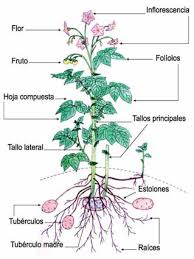
\includegraphics[scale=0.8]{planta.jpeg}
	\label{fig:planta}
\end{figure}

Las plantas de papa criolla (\textit{Solanum phureja}) suelen ser sembradas en calles separadas por una determinada distancia que es lo que se conoce como la densidad de siembra y generalmente con espacios entre surcos de un metro (Bernal, 2017). En la figura \ref{fig:surcos} son identificadas las calles y los surcos en un sembradío. \\

\begin{figure}[h]
	\caption{Sembradío de \textit{Solanum phureja}.}
	\centering
	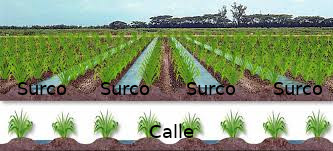
\includegraphics[scale=1]{surcos.jpeg}
	\label{fig:surcos}
\end{figure}

En los cultivos de papa criolla (\textit{Solanum phureja}) son muchas las variables que influyen en la cosecha de los tubérculos, tales como la temperatura, la altura del terreno, el clima, el tipo y la composición del suelo, la densidad de siembra, entre otros. Y de ellas dependen el crecimiento de los tubérculos producidos por la planta (Bernal, 2017). Las variables que influyen en el rendimiento de la papa pueden ser observados en la figura \ref{fig:variablesPapa}. \\

\begin{figure}[h]
	\caption{Variables de influencia sobre el rendimiento de \textit{Solanum phureja}.}
	\centering
	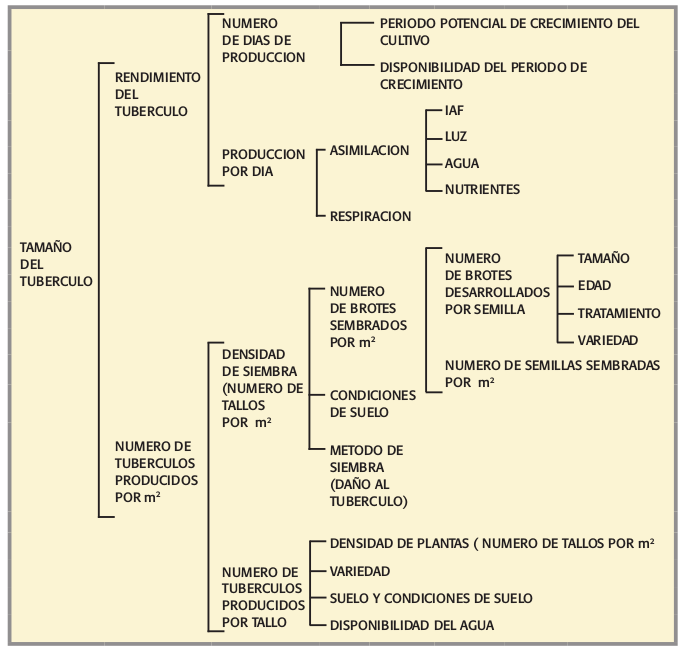
\includegraphics[scale=0.5]{variables.png}
	\label{fig:variablesPapa}
\end{figure}


\subsection{Redes neuronales artificiales.}

Una red neuronal artificial,  es un conjunto de nodos de un programa (neuronas) interconectados entre si, simulando el proceso de pensamiento humano, se pudiera considerar como una caja negra entrenada previamente para esperar una entrada y basado en las características o comportamiento de la misma proporcionar una determinada salida, eliminando así la necesidad de diferentes algoritmos que deban analizar comportamientos cada uno por separado (Stephen, 2007).\\

Entre las definiciones más recientes de inteligencia artificial se expresa, en forma general, la inteligencia artificial como la capacidad que tienen las máquinas para realizar tareas que en el momento son realizadas por seres humanos; otros autores como Nebendah (1988) y Delgado (1998) dan definiciones más completas y las definen como el campo de estudio que se enfoca en la explicación y emulación de la conducta inteligente en función de procesos computacionales basados en la experiencia y el conocimiento continuo del ambiente. Autores como Marr (1977), Mompin (1987), Rolston (1992), en sus definiciones involucran los términos de soluciones a problemas muy complejos.\\

El nacimiento de la inteligencia artificial se sitúa en los años cincuenta; en esa fecha la informática apenas se había desarrollado, y ya se planteaba la posibilidad de diseñar máquinas inteligentes. Hoy en día se habla de vida artificial, algoritmos genéticos, computación molecular o redes neuronales. En algunas de estas ramas los resultados teóricos van muy por encima de las realizaciones prácticas.\\

A través de los años, se han utilizado diversas técnicas de inteligencia artificial para emular ``comportamientos inteligentes''. Al software que hace uso de dichas técnicas se le denomina, de forma genérica, ``sistema inteligente'', y es cada vez más amplia la gama de aplicaciones donde incide la inteligencia artificial.\\

Las redes neuronales artificiales son eficientes en tareas tales como: el reconocimiento de patrones, problemas de optimización o clasificación, y se pueden integrar en un sistema de ayuda a la toma de decisiones, pero no son una panacea capaz de resolver todos los problemas: todo lo contrario, son modelos muy especializados que pueden aplicarse en dominios muy concretos.\\

Las redes neuronales emulan la estructura y el comportamiento del cerebro, utilizando los procesos de aprendizaje para buscar una solución a diferentes problemas; son un conjunto de algoritmos matemáticos que encuentran las relaciones no lineales entre conjuntos de datos; suelen ser utilizadas como herramientas para la predicción de tendencias y como clasificadoras de conjuntos de datos. Se denominan neuronales porque están basadas en el funcionamiento de una neurona biológica cuando procesa información.

\subsection{Redes neuronales probabilísticas.}

Las redes neuronales se utilizan para referirse a una amplia clase de modelos y algoritmos. Las neuronas ocultas se generan en base a alguna combinación de los datos observados, similar a una expansión de base en otras técnicas estadísticas. Sin embargo, en lugar de elegir la forma de la expansión, los pesos utilizados para crear las neuronas ocultas se calculan a partir de los datos. Las redes neuronales pueden implicar una variedad de funciones de activación, que son las transformaciones de las entradas de datos brutos ponderados para crear las neuronas ocultas (Wiley, 2016).\\

Una red neuronal probabilística (PNN) no es mas que una ANN que usa funciones estadísticas que escalan la variable no linealmente como una forma de campana o una distribución normal (Stephen, 2007).\\

Una opción común para las funciones de activación de las redes neuronales es la función sigmoide: $\sigma\left(x\right)=\frac{1}{1+e^{-x}}$ y la función tangente hiperbólica $f\left(x\right)=tanh(x)$. Sin embargo para las redes neuronales probabilísticas que la decisión de cada una de sus neuronas está basada en probabilidades se suelen usar funciones de base radial y aunque suelen existir una variedad de ellas, las PNN usan la forma \textit{Gaussiana}: 

\[
 f\left(x\right) = exp(-\frac{|| x-c ||^2}{2\sigma^{2}})
 \]

\subsection{Curvas ROC.}

Una amplia gama de tests diagnósticos reportan sus resultados cuantitativamente, utilizando escalas contínuas. El análisis de curvas ROC ( \textit{receiver operating characteristic curve}) constituye un método estadístico para determinar la exactitud diagnóstica de estos \textit{tests}, siendo utilizadas con tres propósitos específicos: determinar el punto de corte de una escala continua en el que se alcanza la sensibilidad y especificidad más alta, evaluar la capacidad discriminativa del test diagnóstico y comparar la capacidad discriminativa de dos o más \textit{test} diagnósticos que expresan sus resultados como escalas continuas.

\subsection{Lenguaje R.}

R es un conjunto integrado de \textit{software} de código abierto para el almacenamiento, manipulación, cálculo y visualización de datos para computación y gráficación estadística, puede ser compilado y ejecutado en Windows, Mac OS X y otras plataformas UNIX (como Linux), se distribuye usualmente en formato binario (\url{https://www.r-project.org/about.html}, 2018). El proyecto de \emph{software} R fue iniciado por Robert Gentleman y Ross Ihaka. El lenguaje fue influenciado por  lenguaje S desarrollado originalmente en \textit{Bell Laboratories} por John Chambers y sus colegas. Desde entonces ha evolucionado  para el cálculo estadístico asociado a diversas disciplinas para contextos académicos y comerciales. En R, la unidad fundamental de código compartible es el paquete, el cual agrupa código, datos, documentación y pruebas, y resulta simple de compartir con otros. Para enero del 2015 ya habían más de 6.000 paquetes disponibles en la Red Integral de Archivos de R, conocido comúnmente por su acrónimo CRAN, el cual es el repositorio de paquetes . Esta gran variedad de paquetes es una de las razones por las cuales R es tan exitoso, pues es probable que algún investigador o académico ya haya resuelto un problema en su propio campo usando esta herramienta, por lo que otros usuarios simplemente podrán recurrir a ella para su uso directo o para llamarla en un nuevo código (Wickham,2015). \\

\subsection{Estructura de paquetes en R/RStudio.}

Los requerimientos de núcleo (\textit{core}) para que un desarrollo de software pueda considerarse y compilarse como un paquete de lenguaje R debe cumplir con las siguiente estructura.\\

\begin{enumerate}
  \item  DESCRIPTION: metadatos del package.\\
La tarea del archivo \textit{Description} es de gran importancia ya que es en el donde se registra la metadata, las dependencias que utiliza el paquete, la licencia y el soporte en caso de ocurrir errores con el mismo.
La estructura mínima para realizar un paquete en R es la siguiente:

\begin{itemize}
\item Package: mypackage
\item Title: What The Package Does (one line, title case required)
\item Version: 0.1
\item Authors@R: person(``First'', ``Las'', email = ``first.last@example.com'',
\item role = c(``aut'', ``cre''))
\item Description: What the package does (one paragraph)
\item Depends: R ($>=$ 3.1.0)
\item License: What license is it under?
\item LazyData: true
\end{itemize}
  \item \url{R /:} dirección del repositorio donde se encuentra el código del paquete (.R files).\\
Se expondrán las buenas prácticas a la hora de realizar todo nuestro código en R, desde organización de las funciones, estilos de código y nombre de variables 

\textbf{Organizar funciones en R:} aunque se pueden organizar los archivos como se desee, los dos extremos son malos, no colocar todas las funciones en el mismo archivo y no crear un archivo para cada función, aunque si una función es muy grande o tiene mucha documentación se puede dar el caso, los nombres de los archivos tienen que ser significativo y deben de terminar en $.R$.
\begin{itemize}
\item Bien  
\begin{itemize}
     \item fit\_models.R
     \item utility\_functions.R
  \end{itemize}
\item Mal
   \begin{itemize}
      \item foo.r
      \item stuff.r
    \end{itemize}
 \end{itemize}
Se puede recomendar de acuerdo al número de función utilizar prefijo.

\textbf{Nombres de Objetos:} Los nombres de las variables y funciones deben de ser en min\'usculas, usar el gui\'on bajo ( \_ ) para separar palabras.
\begin{itemize}
\item Bien  
\begin{itemize}
     \item day\_one
     \item day\_1
  \end{itemize}
\item Mal
   \begin{itemize}
      \item first\_day\_of\_the\_month
      \item DayOne
      \item dayone
      \item djm1
    \end{itemize}
 \end{itemize}
En lo posible no usar nombres de variables existentes, ya que esto causar\'a confusi\'on.

\textbf{Espaciado:} Se recomienda colocar espacios alrededor de todos los operadores l\'ogicos y aritm\'eticos (=, +, -, \textless-, etc.). siempre coloque un espacio despu\'es de una coma, y nunca antes de ella.

\begin{itemize}
\item Bien  
\begin{itemize}
     \item average \textless- mean(feet / 12 + inches, na.rm = TRUE)
  \end{itemize}
\item Mal
   \begin{itemize}
      \item average\textless-mean(feet/12+inches,na.rm=TRUE)
   \end{itemize}
 \end{itemize}
 
Hay una pequeña excepci\'on a esta regla: ( :, :: y :::) no necesitan espacios alrededor de ellos.

\begin{itemize}
\item Bien  
\begin{itemize}
     \item x \textless- 1:10
     \item base::get
  \end{itemize}
\item Mal
   \begin{itemize}
      \item x \textless- 1 : 10
     \item base :: get
   \end{itemize}
 \end{itemize}

Dejar un espacio antes del par\'entesis izquierdo, excepto en la llamada a una funci\'on.

\begin{itemize}
\item Bien  
\begin{itemize}
     \item if (debug) do(x)
     \item plot(x,y)
  \end{itemize}
\item Mal
   \begin{itemize}
      \item if(debug)do(x)
     \item plot(x, y)
   \end{itemize}
 \end{itemize}

Se utiliza más de un espacio en caso de que esto mejore a la alineaci\'on, por ejemplo:\\
\begin{list}{}{}
\item list(
    \begin{list}{}{} 
       \item total \hspace{3mm}= a + b + c,
       \item mean \hspace{2mm}= (a + b + c) / n
    \end{list}
\item )
\end{list}
No coloque espacios alrededor del c\'odigo entre par\'entesis o corchetes (a menos que haya una coma)
\begin{itemize}
\item Bien  
\begin{itemize}
     \item if (debug)  do(x)
     \item diamonds[5, ]
  \end{itemize}
\item Mal
   \begin{itemize}
      \item if ( debug ) do(x) \textit{\# no espacios alrededor de debug}
      \item x[1,] \textit{\# necesita un espacio despues de la coma}
      \item x[1 ,] \textit{\# el espacio va despues de la coma no antes}	   
\end{itemize}
 \end{itemize}

\textbf{Llaves:} Una llave de apertura nunca debe ir en su propia l\'inea y siempre debe ir seguida de un nueva l\'inea. Una llave siempre debe ir en su propia l\'inea, a menos que sea seguida por otra y siempre sangr\'ia en el c\'odigo dentro de las llaves
\begin{itemize}
\item Bien  
\begin{itemize}
     \item \begin{list}{}{} 
		\item if (y \textless  \hspace{1mm} 0 \&\&  debug) \{
		\begin{list}{}{}
		\item message(``Y es negativo")
		\end{list}
		\item \}	
	    \end{list}

       \item \begin{list}{}{} 
		\item if (y ==  \hspace{1mm} 0 ) \{
		\begin{list}{}{}
		   \item log(x)
		\end{list}
		\item \} else \{
		\begin{list}{}{}
		  \item y \^~  x
		\end{list}
		\item \}	
	    \end{list}
  \end{itemize}
\item Mal
   \begin{itemize}
     \item \begin{list}{}{} 
		\item if (y \textless  \hspace{1mm} 0 \&\&  debug)
		\item message(``Y es negativo")
	    \end{list}

       \item \begin{list}{}{} 
		\item if (y ==  \hspace{1mm} 0) \{
		\begin{list}{}{}
		   \item log(x)
		\end{list}
		\item \}
		\item else \{
		\begin{list}{}{}
		  \item y \^~  x
		\end{list}
		\item \}	
	    \end{list}   
\end{itemize}
 \end{itemize}

Sentencias que son muy cortas esta bien dejarlas en la misma l\'inea.\\
if(y \textless \hspace{1mm} 0 \&\& debug) message(``Y es negativo")\\

\textbf{Longitud de L\'inea:} cada l\'inea debe de llevar m\'aximo 80 carateres, si se queda sin espacio es recomendable utilzar una funci\'on separada\\

\textbf{Sangria:} Utilize sangria de 2 espacios, nunca use tabulador o multiples tabuladores o espacios. La unica excepci\'on es cuando se define una sentencia en multiples l\'ineas.\\
\begin{tabular}{ccc}
long\_function\_name \textless- function(& a = ``a long argument", \\ 
 &  b = ``another argument", \\
 &  b = ``another argument", \\
\end{tabular}
\newline

\textbf{Asignaci\'on:} Usar el \textless-, y no =
\begin{itemize}
\item Bien  
\begin{itemize}
     \item x \textless- 5
  \end{itemize}
\item Mal
   \begin{itemize}
      \item x = 5
   \end{itemize}
 \end{itemize}

  \item man/: documentación.\\
  \item NAMESPACE: específica que objetos conforman el paquete.\\
\end{enumerate}
\textbf{Comentarios:} Comente su codig\'o, el comentario comienza \#, los comentarios deben de explicar el porque, no el que.\\ Use los caracteres (-) y (=) para separar lineas\\
{\# Load data - - - - - - - - - - - - - - - - - - - - - - - - - - - - - - - - - - - - - -}\\
{\# Plot data - - - - - - - - - - - - - - - - - - - - - - - - - - - - - - - - - - - - - - -}\\


\subsection{RStudio.}

RStudio es un ambiente de desarrollo integrado (\textit{Integrated Development Environment}, IDE) que ofrece herramientas de desarrollo vía consola, editor de sintaxis que apoya la ejecución de código, así como herramientas para el trazado, la depuración y la gestión del espacio de trabajo.  RStudio está disponible para Windows, Mac y Linux o para navegadores conectados a RStudio Server o RStudio Server Pro (Debian / Ubuntu, RedHat / CentOS, y SUSE Linux) (\url{https://www.rstudio.com/about/}, 2018).
 



\chapter{Fundamentos Metodol\'ogicos}

	A continuaci\'on se plantea la estructura a seguir por el presente trabajo, detallando el enfoque, tipo, nivel y dise\~no de la investigaci\'on y la metodolog\'ia a implementar entre otros.
	
\section{Enfoque de la investigaci\'on}
	
	En función de los objetivos planteados en la presente investigación, la misma se adecua a los parámetros de una investigación de tipo proyectivo. La Universidad Pedagógica Experimental Libertador UPEL (2006) expone que la investigación proyectiva consiste en encontrar la solución a los problemas prácticos, se ocupa de cómo deberían ser las cosas para alcanzar los fines y funcionar adecuadamente. Consiste en la elaboración de una propuesta o de un modelo, para solucionar problemas o necesidades de tipo práctico, ya sea de un grupo social, institución, un área en particular del conocimiento, partiendo de un diagnóstico preciso de las necesidades del momento, los procesos explicativos o generadores involucrados y las tendencias futuras.\\
	

	
\section{Dise\~no de la investigaci\'on}
	
El diseño de la investigación es la estrategia general que adopta el investigador para responder al problema planteado,  por lo que es vital establecer una correcta secuencia de pasos para elaborar el prototipo de software que dar\'a solución a la problem\'atica principal de la investigación Arias(2012).\\

\section{Fases metodológicas}

\subsection{Desarrollo del paquete en R}

Los pasos a seguir en el desarrollo de esta investigación serán descritos a continuación siendo basados en los antecedentes y estudios realizados y las pautas estándar establecidas para la creación de paquetes y extensiones en R.\\

\noindent
\textbf{Creación del esqueleto del paquete.}\\
En esta etapa se diseñaran y crearan los directorios, ficheros y objetos que conformaran el paquete.\\

\noindent
\textbf{Registrar el método para el envío y uso de funciones.}\\

Es esta etapa del desarrollo se establecerán las dependencias sobre los paquetes de la base fuente de código R y sus métodos de conexión, considerando el manejo de versiones y los criterios de mantenimiento, además  se establecerán  los espacios de nombre o las estrategias para la búsqueda y utilización de las variables; unificando estos criterios a las funciones que serán diseñadas.\\

\noindent
\textbf{Diseño y codificación de las funciones.}\\

Los m\'etodos para el dise\~no de las funciones primarias en R ser\'an los diagramas de flujo; y para su codificaci\'on se seguir\'an las normas de estilo para codificaci\'on en R, sugeridas por Wickham (2015) y por el creador del paquete \emph{formatR} Xie(2017), adem\'as se establecer\'an la dependencia con las funciones de c\'odigo base y las recomendadas para desarrollo en R.\\

\noindent
\textbf{Explorar y manipular la data.}\\

Los datos tomados de la investigación de Bernal(2017), son datos reales observados de un cultivo de tubérculos de papa criolla que no han sido tratados estadísticamente o modelados, es por eso que en esta etapa se diseñara un algoritmo para la carga de los mismos en estructuras de datos en R.\\

\noindent
\textbf{Diseñar y entrenar la red neuronal probabilística.}\\

En esta etapa se definirán las variables de entrada y se declararan las neuronas patrones y las clases de salida que permitirán la clasificación, para proceder con el entrenamiento de la red que se hará a través del método de \textit{jackknifing} para determinar el parámetro de escalamiento correcto que permita la mejor clasificación.\\

\noindent
\textbf{Pruebas unitarias de las funciones.}\\

Debido a que los paquetes en R están conformados, entre otros elementos por las funciones primarias, a cada una de ellas se les realizaran pruebas unitarias en dos fases, la primera con datos sintéticos que permitan comprobar cada estado del diagrama de flujo, que esquematiza la solución numérica y/o lógica que permite la construcción de a PNN y su entrenamiento. Entre las herramientas ha utilizarse se encuentran los paquetes de R\emph{RUnit} (Zenka, 2015) y \emph{testthat} (Wickham, 2017), y la segunda etapa donde se realizaran las pruebas funcionales del paquete con el conjunto de datos de prueba que formaran parte integral del paquete y con los cuales se desarrollaran los ejemplos prácticos que conformaran la documentación que acompaña al paquete R.\\

\noindent
\textbf{Implementar y realizar pruebas de clasificación.}\\

El objetivo de esta etapa es definir los casos de entrenamiento y prueba que serán usados para buscar la mejor clasificación de densidad de siembra de tubérculos de papa criolla  ante diferentes escenarios.\\

 
  
\noindent
\textbf{Chequear la carga del paquete.}\\

En esta etapa del desarrollo se utilizaran las funciones de chequear paquete que ofrece el código R; cuya finalidad es verificar cada fichero del árbol de carpetas asociadas a cada elemento de la estructura o esqueleto del paquete, que a su vez creara el archivo de documentación en LaTeX y/o HTML, compilará el código fuente y creará las librerías de enlace dinámico (\emph{dynamic link library} DLL).\\  

\noindent
\textbf{Construcci\'on del m\'etodo de distribuci\'on del paquete.}\\

Se seleccionara la forma de distribución del paquete desde el repositorio local, creando los ficheros fuentes  (en formato  \emph{tarball})  y en binario.\\


\subsection{Comparación de resultados.}

En este paso se procederá a la construcción de las curvas ROC asociadas a los casos de prueba planteados para el paquete desarrollado, permitiendo concluir de forma descriptiva  sobre  relaciones entre variables, el mejor manejo de los datos.\\


\section{Aspectos administrativos}

\vspace{1 cm}
La realización de la investigación será planificada según lo establecido en el siguente diagrama:\\

\begin{figure}[!ht]
\begin{center}

\begin{ganttchart}[y unit title=0.4cm,
y unit chart=0.5cm,
vgrid,hgrid,
title height=1,
bar/.style={draw,fill=cyan},
bar incomplete/.append style={fill=yellow!50},
bar height=0.7]{1}{16}
 \gantttitle{Semanas}{16}\\
 \gantttitle{Julio}{2}
 \gantttitle{Agosto}{4} 
 \gantttitle{Septiembre}{4}
 \gantttitle{Octubre}{5}\\
 \gantttitle{Noviembre}{1}\\
 \gantttitlelist{1,...,2}{1}
 \gantttitlelist{1,...,4}{1}
 \gantttitlelist{1,...,4}{1} 
 \gantttitlelist{1,...,5}{1} 
 \gantttitlelist{1,...,1}{1}\\
 \ganttbar{\tiny{Determinación de los lineamientos para el diseño del paquete}}{1}{1} \\
 \ganttbar{\tiny{Creación del esqueleto del paquete}}{2}{2} \\
 \ganttbar{\tiny{Dise\~no de los algoritmos para la biblioteca de funciones}}{2}{3} \\
 \ganttbar{\tiny{Codificación de la biblioteca de funciones}}{3}{9} \\
 \ganttbar{\tiny{Explorar y manipular la data}}{3}{4} \\
 \ganttbar{\tiny{Diseñar y entrenar la red neuronal probabilística}}{5}{8} \\
 \ganttbar{\tiny{Implementar y realizar pruebas de clasificación.}}{8}{12} \\
 \ganttbar{\tiny{Comparación de resultados}}{12}{14} \\
 \ganttbar{\tiny{Graficar y documentar resultados}}{15}{16} \\
 \ganttbar{\tiny{Prueba de la biblioteca de funciones}}{9}{12} \\
 \ganttbar{\tiny{Documentación del paquete}}{4}{12} \\
 \ganttbar{\tiny{Chequeo del paquete}}{10}{14} \\
 \ganttbar{\tiny{Creación del método de distribución del paquete}}{14}{15} \\
 \ganttbar{\tiny{Pruebas de distribución del paquete}}{15}{16} \\
 \ganttbar{\tiny{Realización del informe del proyecto especial de grado}}{2}{16} \\
\end{ganttchart}

\end{center}
\caption{Diagrama de Gantt con la planificación del proyecto especial de grado}
\end{figure}
\chapter{Desarrollo}

	A continuaci\'on se describe de forma detallada, el diseño y desarrollo del paquete \textbf{apnnClassifier} disponible en: \url{ https://github.com/ghouljd/apnnClassifier } para la clasificaci\'on de tub\'erculos de papa criolla(\textit{Solanum phureja}) para diferentes densidades de siembra empleando redes neuronales probabil\'isticas, siguiendo la metodolog\'ia descrita en el Cap\'itulo 3.
	
\section{Creación del esqueleto del paquete.}
	
	Para esta fase se utilizó el ambiente de desarrollo RStudio, el cual es un entorno integrado de fuente abierta para R que agrega muchas caracter\'isticas y herramientas de productividad, además de facilitar el uso de R integrando la ayuda y la documentación.\\

En esta primera etapa se creó la estructura del paquete, la cual está conformada por la identificación por nombre y descripción del paquete (Figura 4.1), además, se cargan los paquetes del CRAN de R y sus extensiones, de los cuales dependen los métodos y funciones que permitiran el desarrollo del paquete \textbf{apnnClassifier}; los mismos fueron almacenados en el repositorio local que se crea para este paquete durante el proceso de desarrollo; los principales fueron:\\

\begin{itemize}
\item pnn(Chasset, P. \textit{et. al}, 2013;\url{https://cran.r-project.org/web/packages/pnn/index.html})
\item pROC(Robin, X. \textit{et. al}, 2019; ;\url{https://cran.r-project.org/web/packages/pROC/index.html})
\item dplyr(Wickham, H. \textit{et. al}, 2019;;\url{https://cran.r-project.org/web/packages/dplyr/index.html})
\item roxygen2(Ooms, J. \textit{et. al}, 2018;;\url{ https://cran.r-project.org/web/packages/roxygen2/index.html})
\end{itemize}

\begin{figure}[h!]
	\caption{Descripción del paquete}
	\centering
	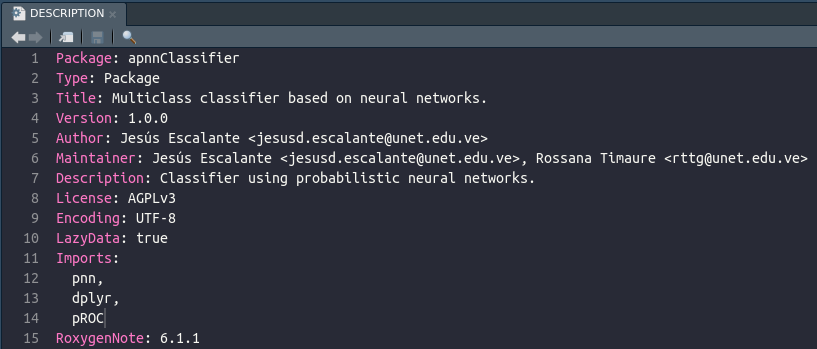
\includegraphics[scale=0.6]{package-description.png}
	\label{fig2:arch}
\end{figure}

\section{Diseño de las soluciones algorítmicas.}

\subsection{Diseño de las soluciones algorítmicas para el entrenamiento de una red neuronal probabilística que permita la clasificación de tubérculos de papa.}

	El objetivo funcional del paquete desarrollado es permitir al usuario realizar el entrenamiento de una red neuronal probabilística para la clasificación de datos estandarizados o no estandarizados, así como graficar y evaluar los resultados de la clasificación.\\

	Para este fin se desarrollaron 2 funciones, necesarias para llegar a los resultados esperados y una opcional para estandarizar los datos de entrada. \\

	Como entrada para iniciar el proceso de entrenamiento y clasificación, es necesario tener un  conjunto de datos de entrenamiento en una estructura \textit{ data.frame}, teniendo conocida cual es la columna que identifica las clases del conjunto; así como tener un conjunto de datos de entrenamiento en forma de matriz con la misma cantidad de columnas como variables clasificadoras tenga el conjunto de entrenamiento.\\

	Las funciones antes mencionadas junto a sus entradas, salidas y diagramas de flujos serán descritas a continuación.\\


\subsection{Diseño del algoritmo de la función de entrenamiento y clasificación de la red (trainNeuralNet).}

	Para el caso de la creación y entrenamiento de la red neuronal probabilística para permitir la clasificación de los datos, se diseñó el ingreso de los datos en dos conjuntos de datos, uno de entrenamiento con la columna de clase incluida y un conjunto de pruebas con la misma cantidad de datos de entrenamiento que el primer conjunto, además de, el índice de la columna indicadora de clase en el conjunto de entrenamiento y el valor óptimo de la función de activación en caso de conocerse (Cuadro \ref{tabla:entradasTrainNeuralNet}.). La función diseñada hace uso del paquete \textbf{PNN} (Chasset, P) de R para crear y entrenar una red neuronal probabilística, el algoritmo de la función se encarga de crear, entrenar, optimizar y clasificar los datos del conjunto de pruebas recibido, obteniendo al final una red neuronal entrenada capaz de clasificar y lista para ser evaluada junto a su clasificación (Figura \ref{fig:trainNeuralNet}).\\

\begin{table}[htb]
\begin{center}
\begin{tabular}{|p{3cm}|p{5cm}|p{8cm}|}
\hline
\multicolumn{3}{|c|}{\textbf{Entradas}} \\
\hline
\textbf{Nombre} & \textbf{Descripción} & \textbf{Reglas} \\
\hline \hline
train\_set & Conjunto de entrenamiento & Parámetro de tipo \textit{data.frame}. Requerido. \\ \hline
test\_set & Conjunto de pruebas & Parámetro de tipo \textit{matriz}. Requerido. \\ \hline
category\_column & Índice de la columna que identifica la categoría o clase en el conjunto de entrenamiento & Parámetro de tipo \textit{entero}. No requerido. Valor por defecto: 1. \\ \hline
sigma & Valor óptimo de la función de activación & Parámetro de tipo \textit{flotante}. No requerido. Es calculado en caso de ausencia del parámetro. \\ \hline
\end{tabular}
\caption{Entradas de la función de entrenamiento - \textbf{trainNeuralNet}.}
\label{tabla:entradasTrainNeuralNet}
\end{center}
\end{table}

\begin{figure}[h!]
	\caption{Diagrama de flujo para función de entrenamiento y clasificación de la red neuronal probabilística}
	\centering
	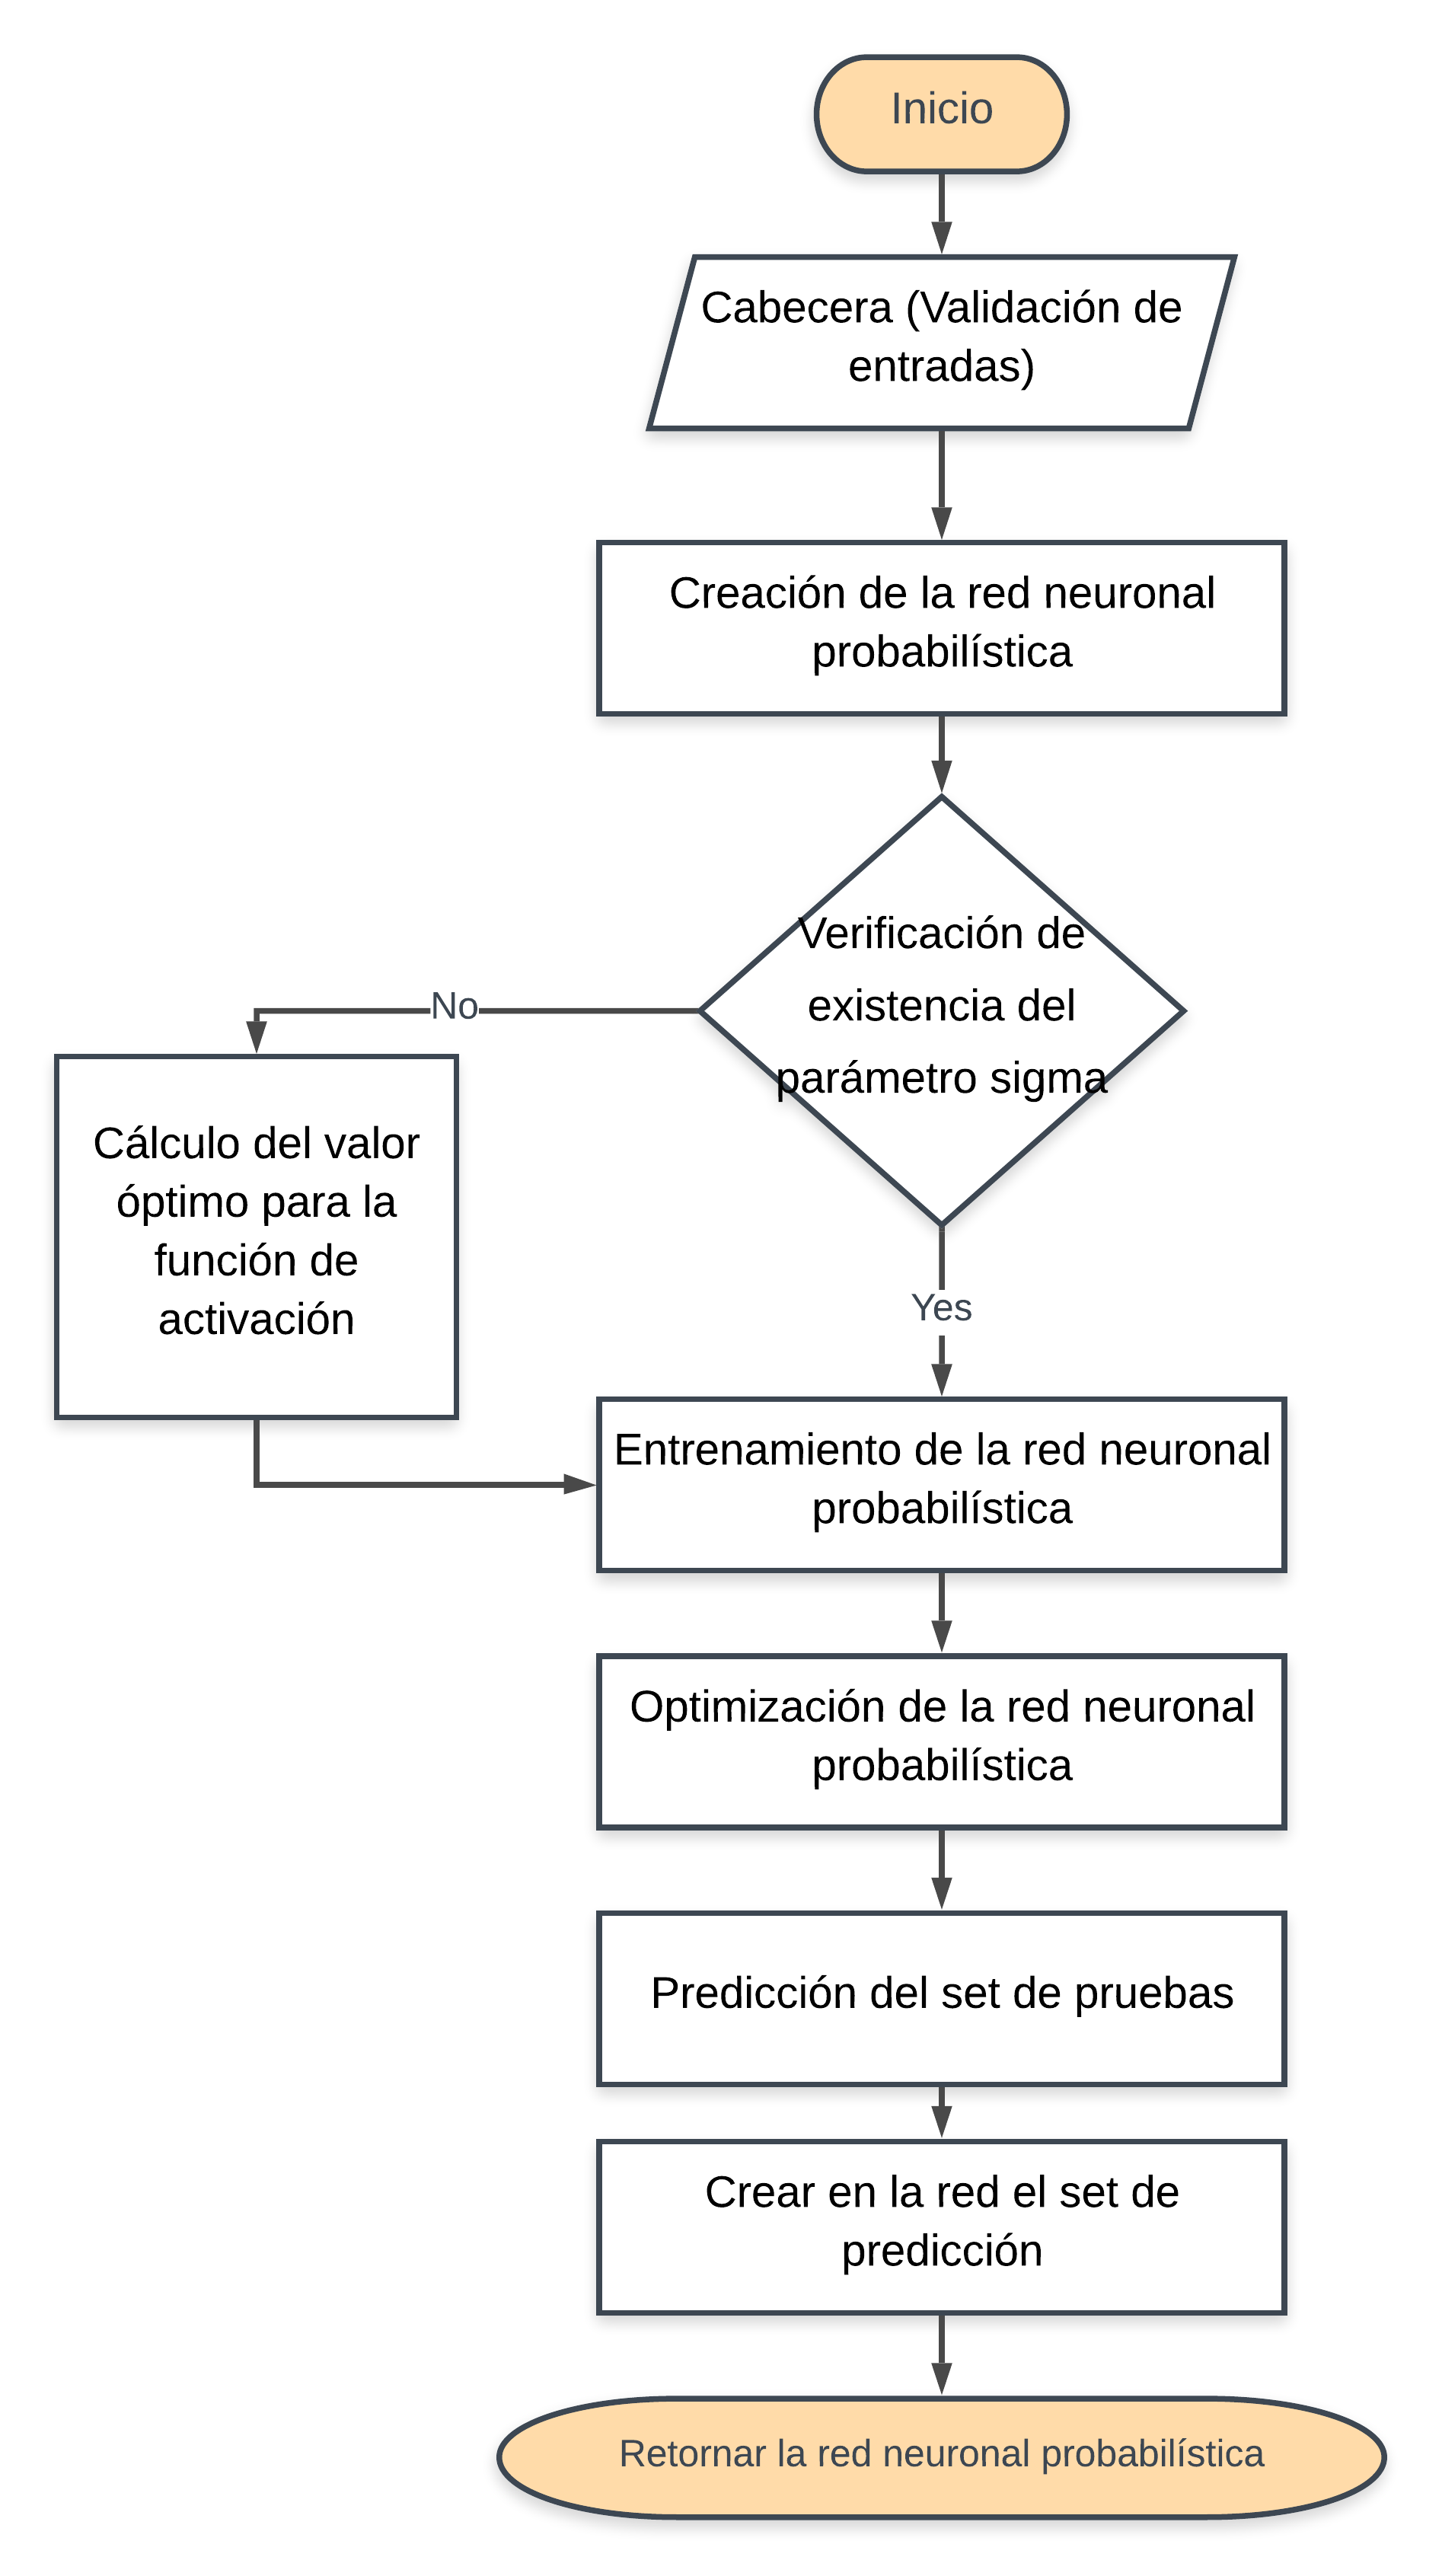
\includegraphics[scale=0.18]{trainNeuralNet.png}
	\label{fig:trainNeuralNet}
\end{figure}

\subsection{Diseño del algoritmo de la función de evaluación de la red neuronal probabilística y su clasificación (evaluate).}

	Para el caso de la evaluación de la red neuronal probabilística y su clasificación, se unificó el ingreso de los datos en la lista de R que se traduce a la red neuronal probabilística que es salida de la función \textbf{trainNeuralNet}, descrita anteriormente (Cuadro \ref{tabla:entradasEvaluate}). La función diseñada realiza la creación del gráfico de nubes de puntos, para demostrar la correlación entre las variables de entrenamiento y hace uso del paquete \textbf{pROC} (Robin, X) de R para crear el gráfico de curvas características operativas (Curvas ROC) para identificar si la clasificación fue buena, el algoritmo también permite observar datos de análisis de la red como su sensibilidad, efectividad y área bajo la curva, para determinar un mal o un buen análisis (Figura \ref{fig:evaluate}. ).\\

\begin{table}[htb]
\begin{center}
\begin{tabular}{|p{3cm}|p{5cm}|p{8cm}|}
\hline
\multicolumn{3}{|c|}{\textbf{Entradas}} \\
\hline
\textbf{Nombre} & \textbf{Descripción} & \textbf{Reglas} \\
\hline \hline
pnn & Red neuronal probabilística & Parámetro de tipo \textit{lista}, que es salida de la función descrita en la sección 4.3. Requerido. \\ \hline
\end{tabular}
\caption{Entradas de la función de evaluación - \textbf{evaluate}.}
\label{tabla:entradasEvaluate}
\end{center}
\end{table}

\begin{figure}[h!]
	\caption{Diagrama de flujo para función de evaluación de la red neuronal probabilística}
	\centering
	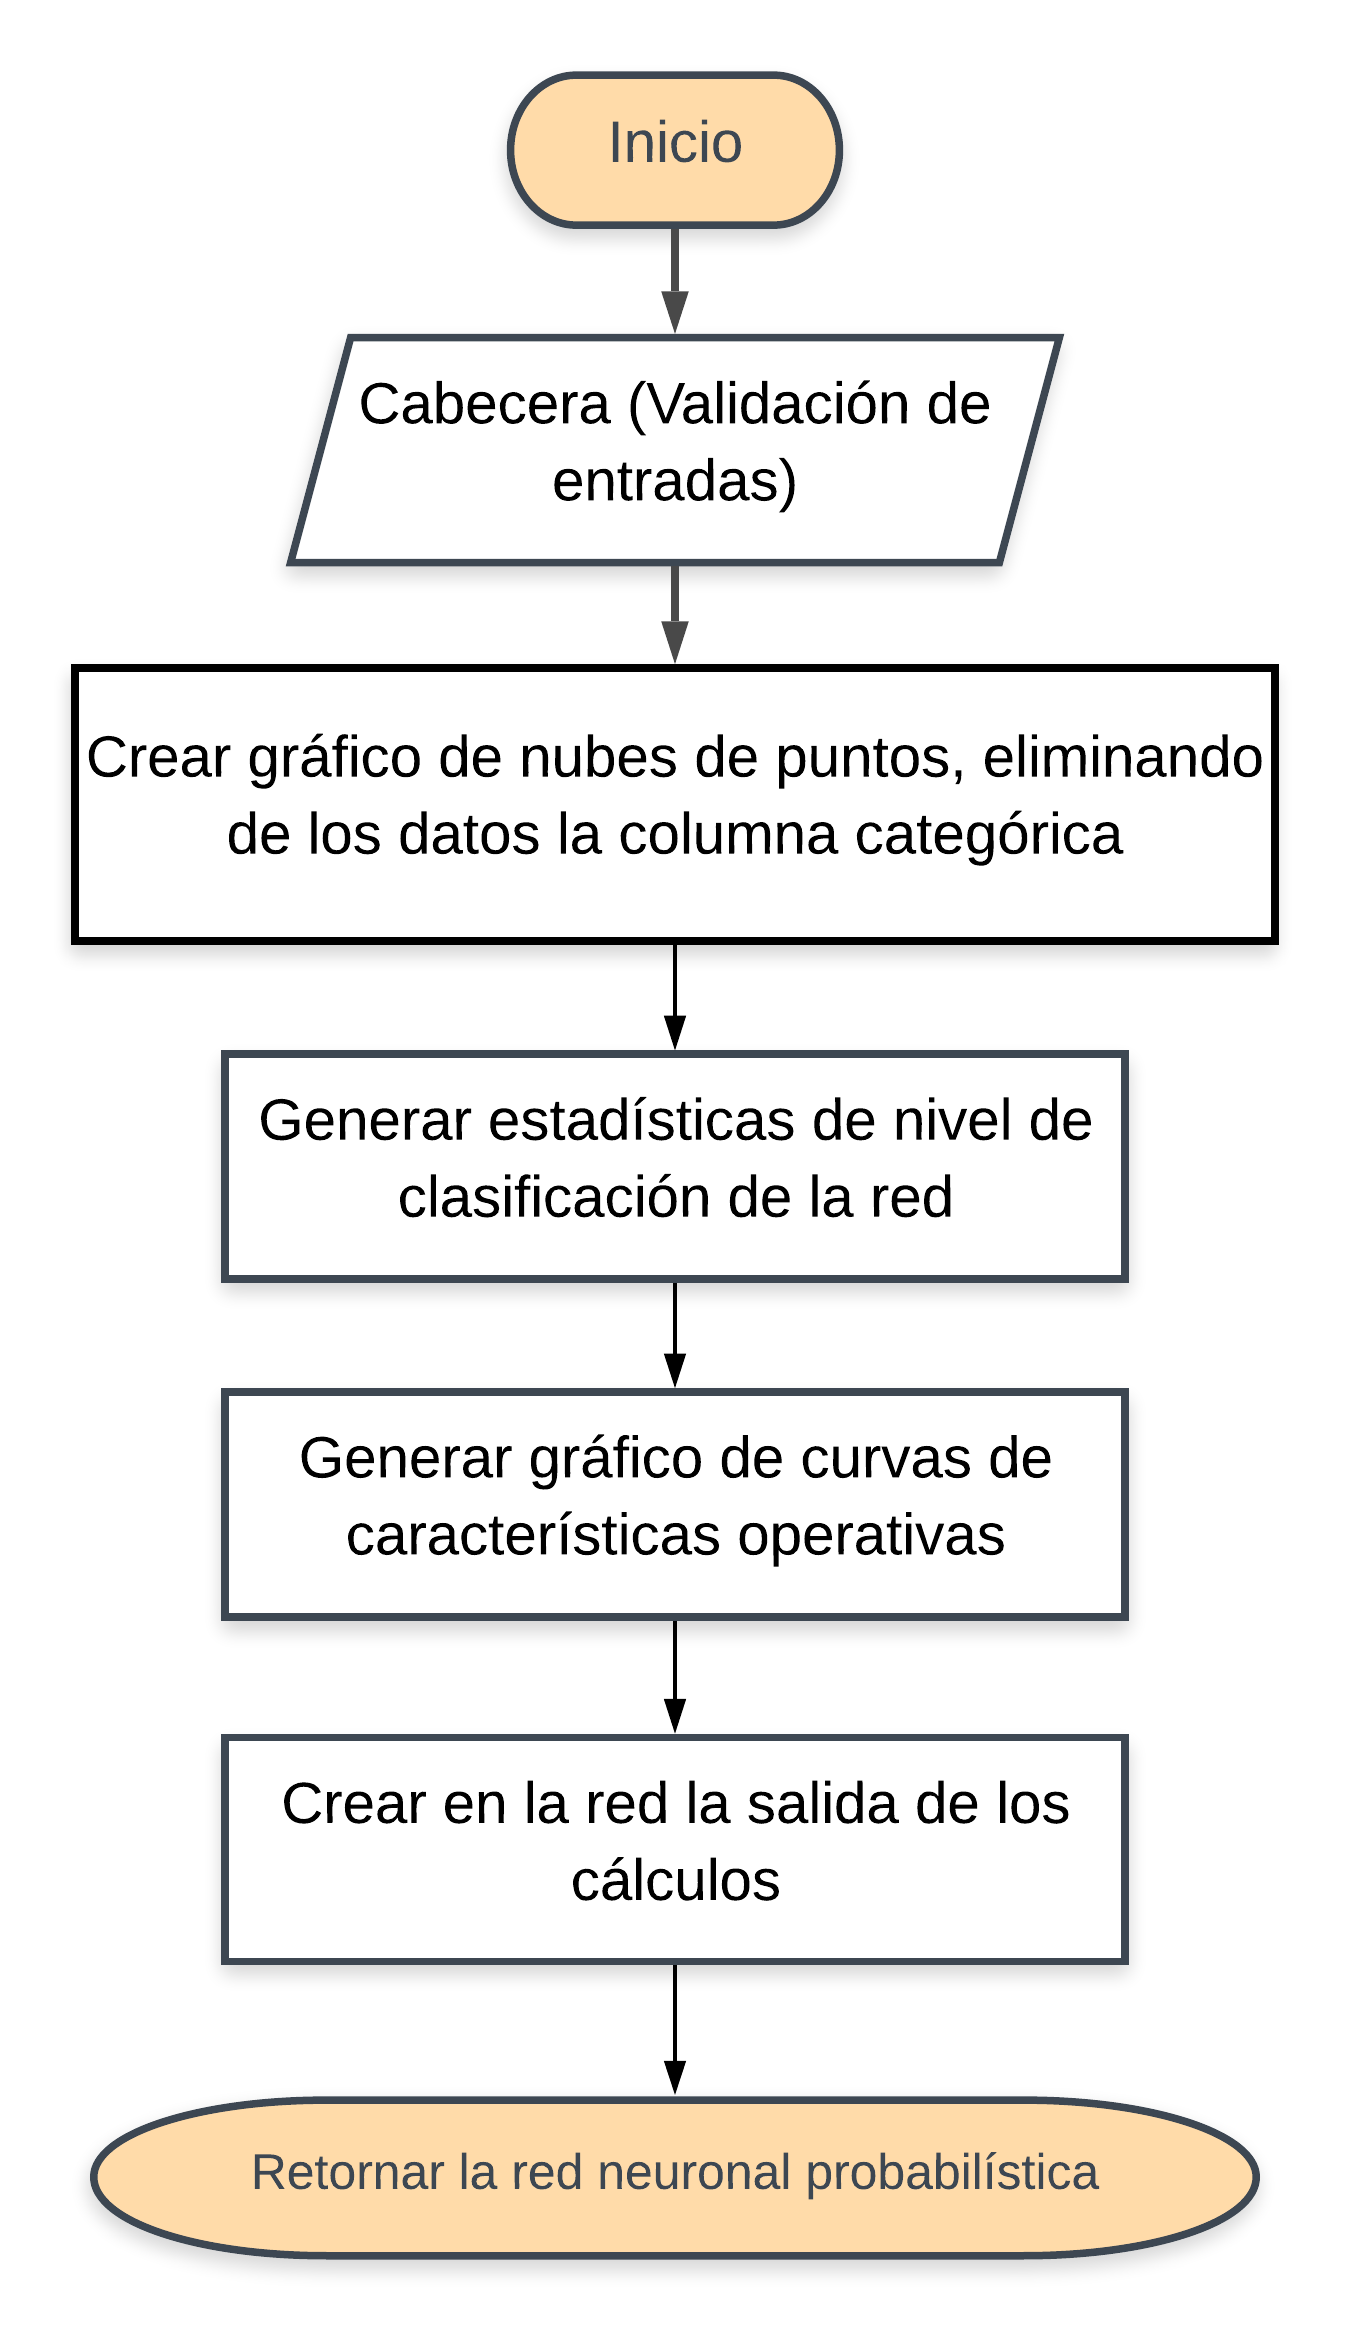
\includegraphics[scale=0.8]{evaluate.png}
	\label{fig:evaluate}
\end{figure}

	La predicción del conjunto de pruebas se puede observar en el atributo “output” de la red neuronal devuelta por la función y es un \textit{data.frame} con dos columnas, una que tiene la predicción y otra con la probabilidad con la que se obtuvo dicha predicción, como se puede observar en la figura \ref{fig:outputTesting}. \\
	
\begin{figure}[h!]
	\caption{Ejemplo de predicción de set de pruebas.}
	\centering
	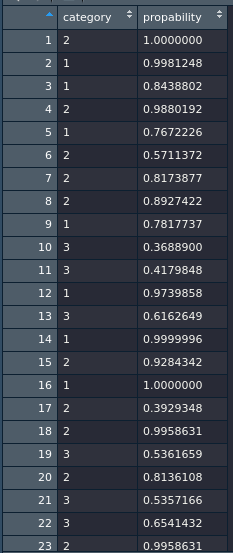
\includegraphics[scale=0.8]{outputTesting.png}
	\label{fig:outputTesting}
\end{figure}

\subsection{Diseño del algoritmo de la función de estandarización de datos (standardize).}

	Para el caso de la estandarización opcional de los datos, se diseñó el ingreso de los datos en un conjunto en formato \textit{lista} o \textit{data.frame}, para este paso se debe tener en cuenta que no tiene sentido alguno estandarizar la columna clase. El tipo de estandarización a usar, que puede ser puntual por media y varianza o escalar por minimos y máximos (Cuadro\ref{tabla:entradasStandardize}). La función diseñada dependiendo del tipo de estandarización indicado en la entrada, aplica la función de estandarización columna por columna del conjunto de datos (figura \ref{fig:standardize}).\\
	
\begin{table}[htb]
\begin{center}
\begin{tabular}{|p{3cm}|p{5cm}|p{8cm}|}
\hline
\multicolumn{3}{|c|}{\textbf{Entradas}} \\
\hline
\textbf{Nombre} & \textbf{Descripción} & \textbf{Reglas} \\
\hline \hline
set & Conjunto de datos & Parámetro de tipo \textit{lista} o \textit{data.frame}. Requerido. \\ \hline
type & Tipo de estandarización & Parámetro de tipo cadena de caracteres. No requerido. Valores posibles: "punctual" - "scale". Valor por defecto: "punctual".\\ \hline
\end{tabular}
\caption{Entradas de la función de estandarización - \textbf{evaluate}.}
\label{tabla:entradasStandardize}
\end{center}
\end{table}

\begin{figure}[h!]
	\caption{Diagrama de flujo para función de  estandarización de datos}
	\centering
	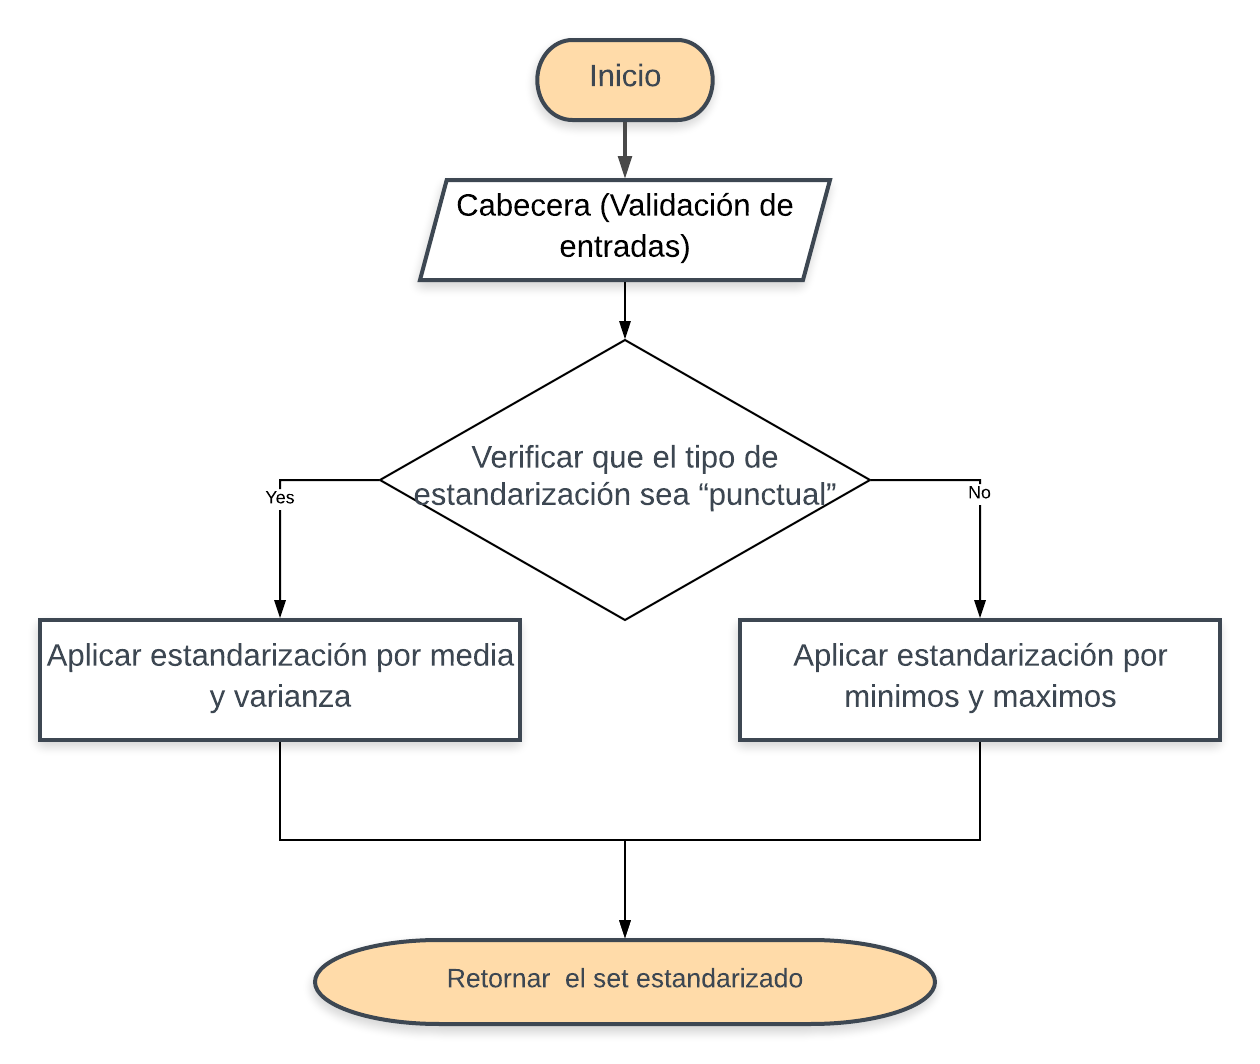
\includegraphics[scale=0.8]{standardize.png}
	\label{fig:standardize}
\end{figure}

\section{Codificación de los algoritmos}

	La codificación de los algoritmos se realizo en el IDE(Entorno de desarrollo integrado) RStudio, siguiendo las especificaciones algoritmicas detalladas con anterioridad.\\

	A continuación se describen las principales funciones creadas para el paquete \textbf{apnnClassifier}.\\
	
\begin{itemize}
\item \textbf{Función de entrenamiento y clasificación de la red \textbf{(trainNeuralNet)}}, crea y entrena una red neuronal probabilística y depende del paquete de R Pnn, la codificación de dicha función se muestra en la figura \ref{fig:codeTrainNeuralNet}.

\begin{figure}[h!]
	\caption{Codificación de la función de entrenamiento y clasificación de la red neuronal probabilística.}
	\centering
	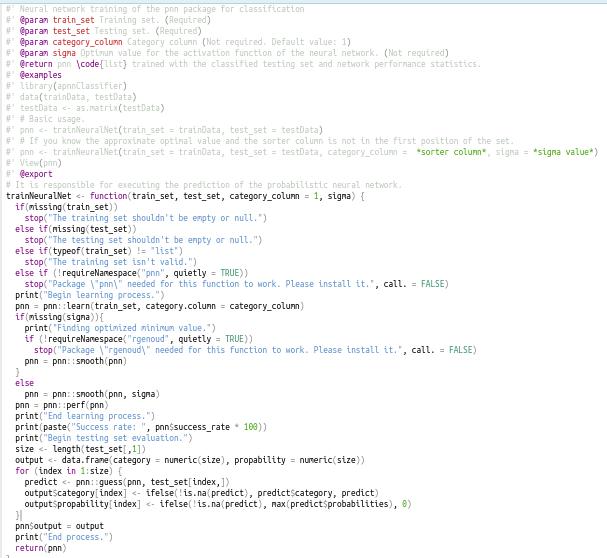
\includegraphics[scale=0.8]{codeTrainNeuralNet.png}
	\label{fig:codeTrainNeuralNet}
\end{figure}

\item \textbf{Función de evaluación de la red \textbf{(evaluate)}}, evalua la especificidad, efectividad y sensibilidad de la clasificación realizada por la red neuronal probabilística y depende del paquete de R \textbf{pROC} y \textbf{dPlyr}, la codificación de dicha función se muestra en la figura \ref{fig:codeEvaluate}.

\begin{figure}[h!]
	\caption{Codificación de la función de evaluación de la red neuronal probabilística.}
	\centering
	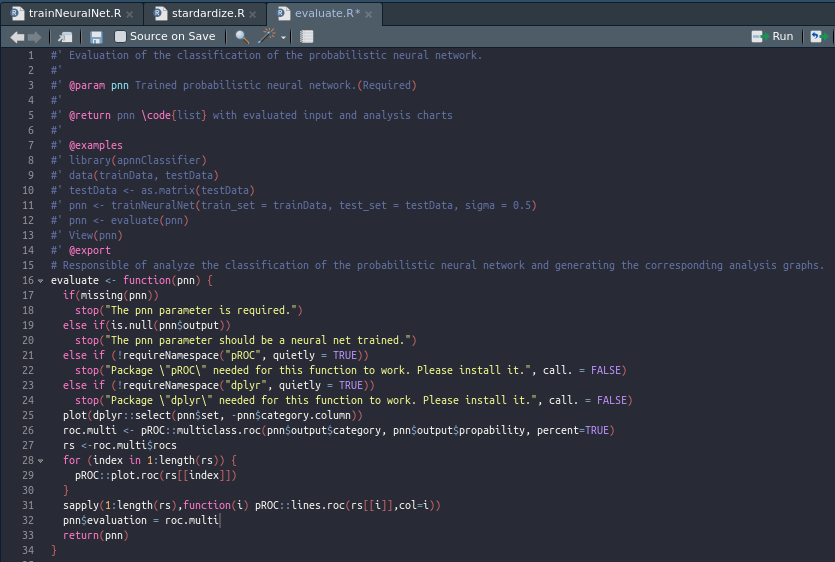
\includegraphics[scale=0.6]{codeEvaluate.png}
	\label{fig:codeEvaluate}
\end{figure}

\item \textbf{Función de estandarización de datos \textbf{(standardize)}}, se encarga de estandarizar los datos basado en dos tipos de estandarización para datos discretos o continuos, la codificación de dicha función se muestra en la figura \ref{fig:codeStandardize}.\\

\begin{figure}[h!]
	\caption{Codificación de la función de estandarización de datos.}
	\centering
	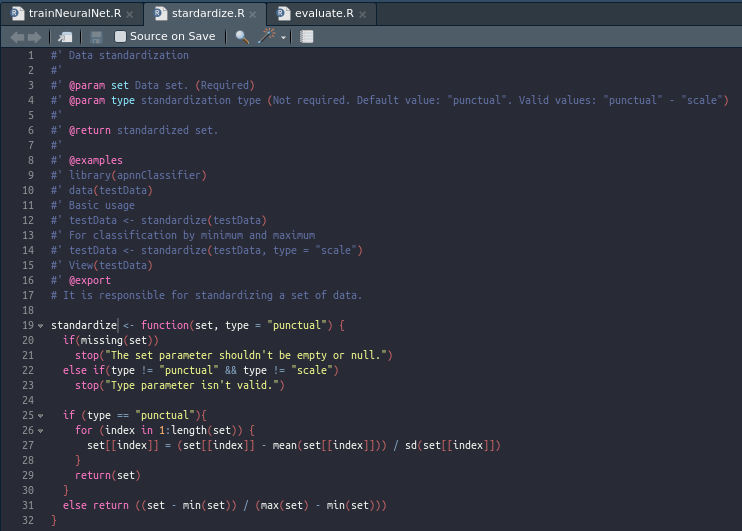
\includegraphics[scale=0.8]{codeStandardize.png}
	\label{fig:codeStandardize}
\end{figure}

\end{itemize}

\section{Chequeo del paquete, método de distribución y registro del método de envío.}

	Para realizar el chequeo del paquete se utilizaron las pruebas unitarias proporcionadas por los paquetes R \textit{RUnit} (Zenka, 2015) y \textit{testthat} (Wickham, 2017). Ver Figura \ref{fig:check}.\\

\begin{figure}[h!]
	\caption{Opción check para realizar el chequeo del paquete.}
	\centering
	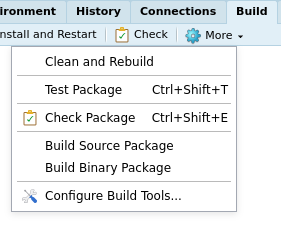
\includegraphics[scale=0.75]{check.png}
	\label{fig:check}
\end{figure}

	Para el método de distribución se utilizara \textit{tar.gz}, que es utilizado por defecto por RStudio. Ver figura \ref{fig:build}. \\
	

\begin{figure}[h!]
	\caption{Opción Build Source Package.}
	\centering
	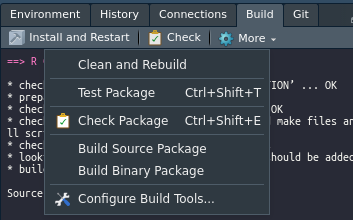
\includegraphics[scale=0.8]{build.png}
	\label{fig:build}
\end{figure}
	
	Como método de envío local se utilizará la plataforma de \textit{GitHub}.\\
	
\section{Pruebas funcionales del paquete}

	El objetivo de este trabajo investigativo consiste en realizar un clasificador de tubérculos de papa criolla para diferentes densidades de siembra y la solución se planteó desarrollando un paquete en R que empleando redes neuronales probabilísticas permitiera dicha clasificación. Para las pruebas funcionales del paquete se realizó la corrida de un algoritmo que permitiera a través del paquete clasificar tubérculos de papa con los datos recogidos en la investigación de Bernal, 2017. \\
	
	Las características que se tomaron para dicha prueba fueron el diámetro medio ponderado, el peso fresco y la cantidad de papas de un conjunto de 2840 datos de campo recogidos en la investigación de Bernal en 2017 (figura \ref{fig:input}). Dicho conjunto de datos fue dividido para la ejecución de las pruebas funcionales en un 75\% para el conjunto de entrenamiento y un 25\% para el conjunto de pruebas. Dicha segmentación se realizó de manera aleatoria por densidad de siembra para asegurar obtener resultados de valor.\\
	
\begin{figure}[h!]
	\caption{Conjunto de datos de entrenamiento.}
	\centering
	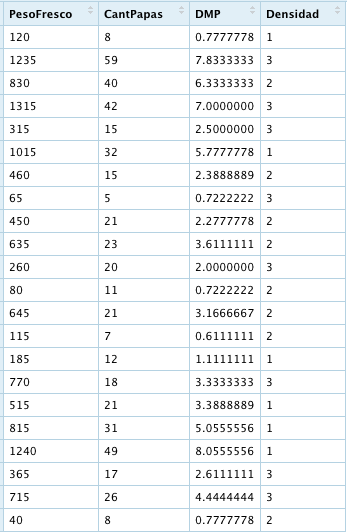
\includegraphics[scale=0.6]{input.png}
	\label{fig:input}
\end{figure}

La codificación de la anterior división, así como el uso de cada una de las funciones del paquete para permitir la clasificación de tubérculos de papa criolla (Solanum phureja) con mencionados conjuntos de datos como entradas se puede observar en la figura \ref{fig:packageuse}.\\

Los resultados obtenidos por el algoritmo se observan en las figuras \ref{fig:cloudpoints} y  \ref{fig:roc}. El concepto de las curvas ROC es contrastar la especificidad (fracción de verdaderos negativos) con la sensibilidad (fracción de verdaderos positivos). Una buena clasificación es caracterizada porque estos dos cálculos se comporten de manera inversamente proporcional, por lo que aunque las correlaciones sean altas entre las variables de entrada como se puede observar en el gráfico de nubes de puntos, no se obtiene una buena clasificación ya que para valores altos de sensibilidad se pueden observar valores altos de especificidad.\\

\begin{figure}[h!]
	\caption{Codificación del algoritmo de clasificación usando \textit{apnnClassifier}.}
	\centering
	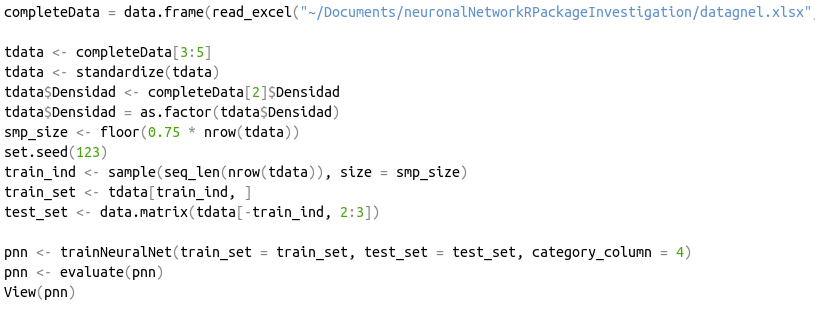
\includegraphics[scale=0.6]{packageuse.png}
	\label{fig:packageuse}
\end{figure}

\begin{figure}[h!]
	\caption{Gráfico de nubes de puntos.}
	\centering
	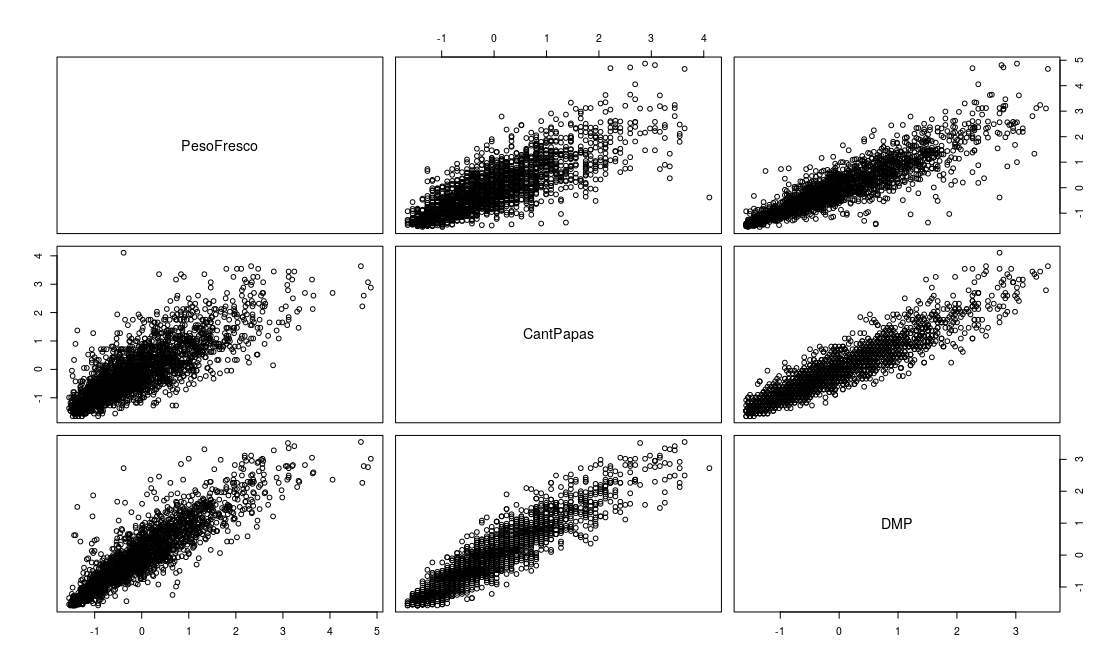
\includegraphics[scale=0.6]{cloudpoints.png}
	\label{fig:cloudpoints}
\end{figure}

\begin{figure}[h!]
	\caption{Gráfico de curva característica operativa de receptor.}
	\centering
	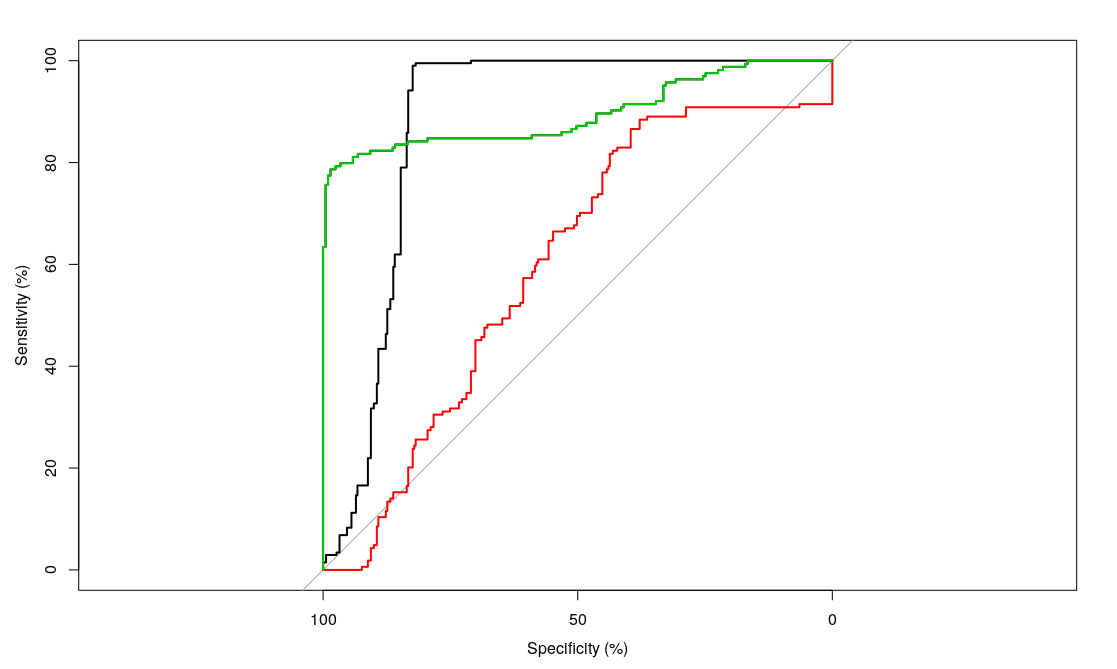
\includegraphics[scale=0.5]{roc.png}
	\label{fig:roc}
\end{figure}
\chapter{Conclusiones y recomendaciones}

	Se diseñaron las soluciones algorítmicas para el entrenamiento de redes neuronales probabilísticas, lográndose ajustar a cualquier tipo de clasificación sin sesgar los algoritmos al objetivo general que es la clasificación de tubérculos de papas, esto con el fin de que el paquete pueda ser usado independiente del tipo de datos que se tengan para clasificar. Se observó que el algoritmo funciona de manera mucho más rápida cuando se conoce o se prueban manualmente valores para el punto óptimo de la función de activación, ya que como cualquier clasificador, para un set de datos grande los tiempos calculando este punto podrían elevarse considerablemente.\\

Se codificaron tres funciones que permiten resolver los algoritmos y la problemática planteada. Estas funciones son parametrizables, permitiendo el entrenamiento de redes neuronales probabilísticas para clasificar cualquier tipo de datos y en tantas clases como se requiera en otras investigaciones independientemente de su complejidad o cantidad de datos. \\

Se realizaron pruebas del paquete comenzando por clasificaciones sencillas con dos entradas y dos clases hasta una cantidad de cinco entradas y tres clases. Determinando así que se realizó un buen clasificador con buenos resultados, pues se evidencian buenas áreas bajo la curva en los gráficos de curvas características. \\

Se concluyó basado en los estudios realizados por Bernal en 2017, que las variables que más afectan la densidad de siembra en los cultivos de papa criolla (Solanum phureja), son el peso fresco, la cantidad de papas por planta y el diámetro medio ponderado. Se recomienda realizar pruebas con otras variables a fin de validar si existen otras combinaciones de parámetros de entrada que brinden una mejor clasificación.\\

Con respecto al análisis realizado con el paquete en la clasificación realizada para los datos de tubérculos de papa realizado por Bernal, 2017, no se obtuvo una buena clasificación, debido a dos razones, los datos fueron tomados mediante conteos afectando la clasificación bajo los supuestos de muestreo, además se puede concluir que aunque exista correlación entre las variables que fueron usadas como entrada al algoritmo (peso fresco, diámetro medio ponderado y cantidad de papas) no son buenos clasificadores para la densidad de siembra. Se recomienda trabajar los datos de entrada estadísticamente, eliminando datos atípicos y probar otros sistemas de muestreo en la recolección de datos con el fin de obtener mejores clasificaciones.\\

Con respecto al desarrollo de software, bajo el paradigma del desarrollo de paquetes en lenguaje R, apnnClassifier es fácilmente escalable, dado que la red neuronal probabilística puede ser parametrizable, debido a que es de código abierto, puede anexarse en nuevas versiones a la
librería de funciones del paquete.\\

Como recomendación, se puede evaluar el desarrollo de un ambiente para gráficos más interactivo con el usuario o en plataforma WEB, elementos que se encontraban fuera del alcance de este proyecto de investigación.\\
%% Los cap'itulos inician con \chapter{T'itulo}, estos aparecen numerados y
%% se incluyen en el 'indice general.
%%
%% Recuerda que aqu'i ya puedes escribir acentos como: 'a, 'e, 'i, etc.
%% La letra n con tilde es: 'n.

\chapter*{Referencias Bibliográficas}

\noindent
Available CRAN Packages By Name. Disponible en:\url{ https://cran.r-project.org/web/packages/available_packages_by_name.html}. Consultada Junio 2018.\\

\noindent
Lanz Brett, Reino Unido. Machine Learning with R. 2015. \\

\noindent
Bohorquez Ingrid, Ceballos Ermilson. Algunos conceptos de la econometría espacial y el análisis exploratorio de datos espaciales. 2008.

\noindent
Stephen Gang Wu, Forrest Sheng Bao, Eric You Xu, Yu-Xuan Wang, Yi-Fan Chang, Qiao-Liang Xiang. A Leaf Recognition Algorithm for Plant Classification Using Probabilistic Neural Network. 2007.

\noindent
Nur Badariah Ahmad Mustafa, Kumutha Arumugam, Syed Khaleel Ahmed, Zainul Abidin Md Sharrif. Classification of Fruits using Probabilistic Neural Networks - Improvement using Color Features. 2011.

Bernal Nelson. Modelado del Calibre y la competición intra-específica por rendimiento de tubérculos de papa variedad Solanum phureja bajo diferentes densidades de siembra. 2017.




%% Incluir la bibliograf'ia. Mirar el archivo "biblio.bib" para m'as detales
%% y un ejemplo.


\end{document}
